%%%%%%%%%%%%%%%%%%%%%%%%%%%%%%%%%%%%%%%%%%%%%%%%%%%%%%%%%%%%%%%%%%%%%%%%%%%%%%%
% intro.tex: Introduction to the thesis
%%%%%%%%%%%%%%%%%%%%%%%%%%%%%%%%%%%%%%%%%%%%%%%%%%%%%%%%%%%%%%%%%%%%%%%%%%%%%%%%
\chapter{Tabulation}
\label{tabulation_chapter}
%%%%%%%%%%%%%%%%%%%%%%%%%%%%%%%%%%%%%%%%%%%%%%%%%%%%%%%%%%%%%%%%%%%%%%%%%%%%%%%%
%To accelerate VLE solvers, we implemented two tabulation methods: traditional lookup table and \textit{in situ} adaptive tabulation. The lookup table is simple and fast but requires more memory, while \textit{in situ} adaptive tabulation can achieve high speedup and control the error and memory usage.

Although the vapor-liquid equilibrium (VLE) model has an incomparable advantage in predicting phase transitions of transcritical flows, the computational cost of VLE calculations can be prohibitively high. We use two tabulation methods to accelerate the calculation of the model, which makes the model calculation greatly optimized. The methods we developed are traditional lookup table and \textit{in situ} adaptive tabulation are discussed in Sec.~\ref{sec:tra-tab} and Sec.~\ref{sec:ISAT}. Moreover, ISAT method is further optimized for parallel computation in Sec.~\ref{sec:pISAT}.

\section{Lookup table} \label{sec:tra-tab} % and its verification

%The new contributions from this study to the OpenFOAM solver and PIMPLE algorithm are summarized here. This study replaces the original thermodynamic model with the VLE + PR-EOS model implemented in this study, as shown in Fig.~\ref{FC_CFD}. Due to the high computational cost of VLE calculation, a novel VLE-based tabulation method is developed to accelerate simulations and make the CFD solver computationally more affordable, as shown in the right box of Fig.~\ref{FC_CFD}. For each simulation, a table is generated to record the solution of TP flash, density, enthalpy, $c_p$, and transport properties at different temperatures (280-1200 K), pressures (280-700 bar), and \ce{CO2} mole fractions (0.0001-0.9999). Each solution includes, every species' mole fraction in liquid and gas phases, and transport properties. In simulations, a linear approximation method based on eight neighboring records is used for data retrieval. More details about this VLE-based tabulation method is provided in Appendix~\ref{App:tab}. For a large number of components, this tabulation method will demand infeasible memory, and we are developing a new on-the-fly tabulation of VLE solutions using the \textit{in situ} adaptive tabulation (ISAT) approach \cite{zhang2021multi}, similar to the idea of correlated dynamic evaluation of real fluid properties for supercritical mixing \cite{yang2017comparison} and combustion \cite{milan2019time}.  

%%In the lookup table method, the VLE is computed entirely in the preprocessing phase, which allows expensive computation to be completely avoided. This also allows CFD solver to be completely decoupled from the code implementation of the thermodynamic model. This makes it easy for a single CFD code to use different thermodynamic models without any changing, which is a valuable advantage considering almost all solvers are becoming more complex nowadays. On the other hand, the robustness of some complex thermodynamic models is a huge problem. When doing 0D thermodynamic analysis, occasionally the model solution does not converge, but it will not seriously affect the research. However, in CFD, the non-convergence of the solution is difficult to be automatically captured by the code, in millions of model solutions. Even one model does not converge, can lead to the collapse of the entire simulation. By using lookup table, solving the model is completely in the pre-processing stage, and the above problems can be avoided.

The lookup table method computes Vapor-Liquid Equilibrium (VLE) entirely during the preprocessing phase, effectively eliminating the need for computationally expensive calculations. This decoupling of thermodynamic models from the CFD solver's code implementation offers significant advantages. It simplifies the process of adapting a single CFD code to accommodate various thermodynamic models without requiring code alterations, a crucial advantage in light of the increasing complexity of modern solvers. Furthermore, certain intricate thermodynamic models exhibit limited robustness. While this may not pose a significant issue in the context of 0D thermodynamic analyses, it becomes a pivotal concern in CFD. In CFD solvers, the model must be solved millions of times, and any failure can spell disaster for the entire simulation. The lookup table method elegantly sidesteps these challenges by relegating model solving exclusively to the pre-processing phase.


%%In this work, the lookup table method is used in PIMPLE solver to replace the TP flash calculation. Our method, like most methods, estimates the range of input parameters involved in the simulation. Within the given range of temperature, pressure, and mass fraction, TP problems are solved on the evenly spaced grid points. Then the thermodynamic proprieties (including $\rho$, $h$, $c_v$, $c_p$) and transport proprieties (including $D_m$, $\mu$, $\lambda$) are evaluated using TP solutions. The input values of the table form a evenly distributed structure grid, and the search process can be easily and quickly determined by the range and intervals of the input parameters. 

In our work, we implement the lookup table method in the PIMPLE solver as a replacement for TP flash calculations. Similar to most works, our approach first estimates a range of input parameters according to the simulation we want to conduct. With the given range of temperature, pressure, and mass fraction, a structured grid with uniform intervals is defined. TP problems are solved at these evenly spaced grid points. Subsequently, thermodynamic properties (such as density, enthalpy, specific heat at constant volume, and specific heat at constant pressure) and transport properties (including mass diffusion coefficient, viscosity, and thermal conductivity) are computed using the TP solutions.


%A tabulation method is used to accelerate VLE model computation. This method is used to replace the computationally expensive on-the-fly TP flash. Within the given range of temperature, pressure, and mass fraction, TP problems are solved on the evenly spaced grid points. Then the thermodynamic proprieties (including $\rho$, $h$, $c_v$, $c_p$) and  transport  proprieties (including $D_m$, $\mu$, $\alpha$) are evaluated using TP solutions. 
The TP solutions and all properties are recorded into the table. When retrieving the solution of given input ($T^*$, $p^*$, $x^*$), linear interpolation is used:
\begin{enumerate}
	\item Find the closest temperature, pressure and mass fraction in the table,
	      $T_1 \leq T^* < T_2 $,
	      $p_1 \leq p^* < p_2 $,
	      $x_1 \leq x^* < x_2 $
	\item Calculate the weight for linear interpolation,
	      $ \alpha^v_1=\frac{v_2-v^*}{v_2-v_1}$,
	      $ \alpha^v_2=\frac{v^*-v_1}{v_2-v_1}$, $v=T,p,x$
	\item For any property $A$ in the table, linear interpolation uses the formula $A^* = \sum_{i,j,k=1,2}\alpha^T_i \alpha^p_i \alpha^x_i A_{ijk} $
\end{enumerate}

%%The density of the records in lookup table needs to be considered according to the degree of nonlinearity of the stored model. The accuracy of this method needs to be determined through testing. The accuracy test are conducted when using lookup table methods in Sec.~\ref{sec:results:JICF}. This method has been used in many works and satisfactory results have been obtained \cite{yi2019numerical,jafari2021towards,jafari2022exploring}. 


%%However, this method is difficult to deal with the problem of making more components. The memory requirement of lookup table grows exponentially with the number of components, leading to unaffordable memory demands for larger systems (i.e., the curse of dimensionality: table size $\sim M^N$, where $M$ is the number of grids of each component in the table and $N$ is the number of components). For example, using a table with the same resolution as the one in Sec.~\ref{sec:results:JICF} (e.g., a table with variable range: $T$ 470-600 K, $P$ 9-25 MPa, $x_i$ 0.6-0.9, and interval: $\Delta T = 1.3$ K, $\Delta P = 0.4$ MPa, $\Delta x_i = 0.015$) for a 4-component system, would result in a table size of approximately 4 terabytes (TBs). Storing such large tables in each CPU core (without shared memory) or each node (with shared memory) becomes infeasible for existing computing facilities. Moreover, the tabulation region, which is defined by the upper and lower bounds of each input value, is very crude, and large amounts of data are almost never used. If these redundant data can be removed, the memory consumption can be greatly reduced. We develop a new tabulation method to handle this problem in the next section.


The density of records (intervals of parameters) in the lookup table needs careful consideration in accordance with the nonlinearity of the stored model and the requirement of accuracy. To assess the accuracy of this approach,  testing is imperative, as elaborated in Sec.~\ref{sec:results:JICF} where we employ lookup table methods. This method has garnered commendable results in various  works \cite{yi2019numerical,jafari2021towards,jafari2022exploring}.

Nonetheless, it faces a significant challenge when dealing with systems involving an increasing number of components. The memory requisites for lookup tables burgeon exponentially with the number of components, leading to unaffordable memory demands for larger systems (i.e., the curse of dimensionality: table size $\sim M^N$, where M is the number of grids of each component in the table and N is the number of components). As an illustration, using a table with the same resolution as the one in Sec.~\ref{sec:results:JICF} (e.g., a table with variable range: $T$ 470-600 K, $P$ 9-25 MPa, $x_i$ 0.6-0.9, and interval: $\Delta T = 1.3$ K, $\Delta P = 0.4$ MPa, $\Delta x_i = 0.015$) for a 4-component system simulation, would need a table size of approximately 4 terabytes (TBs). Storing such colossal tables in each MPI process (without shared memory) or each node (with shared memory) becomes utterly impractical given the limitations of current computing facilities.

Furthermore, the tabulation region, defined by the upper and lower bounds of each input parameter, tends to be overly crude,  and a vast portion of the data is seldom utilized. Removing redundant data could substantially alleviate memory consumption. In the subsequent section, we introduce a novel tabulation method designed to address this issue.


\comment{
To mitigate the concern about potential VLE-inconsistency, an accuracy test is provided here. The same shock tube case as the one in Sec.~\ref{sec:results:ShockTube} is used to test the tabulation method. The shock tube condition is shown in Table~\ref{conditions}.
The table used for the simulation covers the temperature range of 470-600 K, pressure range of 9-25 MPa, and $x_{\ce{CO2}}$ range of 0.6-0.9. The table grid sizes are $\Delta T = 1.3$ K, $\Delta p = 0.4$ MPa, and $\Delta x_{\ce{CO2}} = 0.015$.
The $L^{\infty}$ absolute error (i.e., $max(\Delta A)$), maximum local relative error (i.e., $max(\frac{\Delta A}{A})$), and $L^2$ relative error (i.e., $ \frac{\|\Delta A\|_{L^2}}{\|A\|_{L^2}}$) are obtained by comparing to the results without tabulation, and shown in Table.~\ref{table:error}. The results show that the maximum local errors are controlled within 10\% and the $L^2$ errors are control within 5\%.

\begin{table}[htbp]
	%\begin{center}
	\centering
	\begin{minipage}{0.9\textwidth}
		\caption{Relative error of VLE-based tabulation method.} \label{table:error}
		\begin{center}
			\begin{tabular}{@{}l|lll@{}} %\hline
				\toprule
				                             & Pressure & Density        & Gas Mole Frac. \\ %\hline
				\midrule
				$L^{\infty}$ absolute error  & 0.17 MPa & 5.889 $kg/m^3$ & 0.02           \\%\hline
				maximum local relative error & 1.4\%    & 1.6\%          & 2.1\%          \\ %\hline
				$L^2$ relative error         & 0.09\%   & 0.09\%         & 0.1\%          \\ %\hline
				\bottomrule
			\end{tabular}

		\end{center}
	\end{minipage}
	%\end{center}

\end{table}
}

\section{\textit{In Situ} Adaptive Tabulation (ISAT)}
\label{sec:ISAT}
\subsection{introduction}
In flame simulation, a detailed combustion kinetic mechanism often includes tens to hundreds of species and hundreds to thousands of reactions. The simulation of complex flames (e.g., turbulent flames) requires solving many conservation equations, including detailed finite-rate chemistry, which demands a large amount of computational cost. This amount of computation makes flame simulation difficult. Since combustion involves high dimensional data, traditional lookup is impossible. To reduce the computational cost, Pope~\cite{pope1997computationally} introduce \textit{in situ} adaptive tabulation (ISAT).

ISAT is an on-the-fly tabulation method, in which records are dynamically added with additional information (e.g., the gradient of function). ISAT maintains error control by using finer granularity in regions of increased nonlinearity (shown in Fig.~\ref{ISAT_Schematic}). In a combustion simulation, the solution of chemical ordinary differential equations (ODE) is tabulated, which avoids a large amount of repeated computation and obtains a speed-up factor of about 1000 \cite{pope1997computationally}. ISAT has been successfully used in many combustion simulations \cite{pope1997computationally,gordon2007numerical,wang2003application,singer2006modeling,singer2004exploiting,tang2002implementation}. Moreover, several research works have been done to improve the algorithm. Chen improved performance by modifying search algorithm \cite{chen2004analysis}; Lu et al. implemented parallel ISAT in LES \cite{lu2005investigation}; Lu and Pope improved table searching strategies, error checking, and correction algorithms \cite{lu2009improved}; Blasi et al. extended ISAT to accelerate the simulation of complex heterogeneous chemical kinetics \cite{blasi2016situ}. Furthermore, ISAT has demonstrated its adaptability across diverse problem domains, encompassing areas such as chemical engineering \cite{shah1999computational,kolhapure2005pdf,10.1115/1.2709655}, surface reactions \cite{mazumder2005adaptation}, thin film growth \cite{varshney2005multiscale}, solid mechanics \cite{arsenlis2006generalized}, control systems \cite{hedengren2008approximate}, and turbulent combustion models based on manifolds \cite{lacey2021situ}.


\begin{figure}[htbp]
	\centering
	\includegraphics[width=0.80\linewidth]{ISAT schem.png}
	\caption{Schematic of turbulent flame simulation and ISAT.}
	\label{ISAT_Schematic}
\end{figure}

In contrast to traditional tabulation methods that require pre-processing to generate tables before the CFD simulation, ISAT dynamically constructs the table during the simulation. This dynamic construction enables us to store only the necessary records, significantly reducing the table size and mitigating the curse of dimensionality. During the CFD simulation, most of the queries can be efficiently retrieved by utilizing linear approximation based on the table records, eliminating the need for direct calculations. This approach not only enhances computational efficiency but also ensures that the results are obtained with a high degree of accuracy. ISAT's ability to provide excellent error control contributes to maintaining the desired level of precision. Given these advantages, employing the ISAT method to tabulate VLE solutions proves to be a promising strategy for accelerating VLE-based CFD simulations. In this work, we develop an ISAT-based VLE to accelerate VLE calculation.

%The \textit{in situ} adaptive tabulation (ISAT) method, originally introduced by Pope \cite{pope1997computationally}, offers an effective approach to reduce the computational cost associated with detailed chemistry calculations. In contrast to traditional tabulation methods that require pre-processing to generate tables before the CFD simulation, ISAT dynamically constructs the table during the simulation itself. This dynamic construction enables us to store only the necessary records, significantly reducing the table size and mitigating the curse of dimensionality. During the CFD simulation, most of the queries can be efficiently retrieved by utilizing linear approximation based on the table records, eliminating the need for direct calculations. This approach not only enhances computational efficiency but also ensures that the results are obtained with a high degree of accuracy. ISAT's ability to provide excellent error control contributes to maintaining the desired level of precision. Given these advantages, employing the ISAT method to tabulate VLE solutions proves to be a promising strategy for accelerating VLE-based CFD simulations.

%The fluid solver directly updates pressure $P$, enthalpy $h$, and mass mole fraction of every component $Y_m$ from the governing equation, and require thermodynamic model to evaluate temperature $T$, and gas mole fraction $\psi_g$ and speed of sound $c$. ($T$,$\psi_g$) can be solved by PH flash solver, $c$ is obtained from analytical approach \cite{tudisco2020analytical}. 
\subsection{ISAT Method}
In a VLE model, the relation between the given input condition $\boldsymbol{x}$ and output solution $\boldsymbol{y}$ can be denoted as a function or mapping $\boldsymbol{F}$:
$$\boldsymbol{y=F\left(x\right)}.$$
%This functional relationship is determined by the needs of the CFD solver. Specifically, in this work, the FC and DF schemes have different functional relationships.
Specifically, the input and output variables are required for the implementation of the FC and DF schemes. Firstly, the speed of sound $c$ is required for flux splitting schemes. %ensure the accuracy and stability of the solver. 
Additionally, the vapor mole fraction $\beta$ is used for capturing phase separation. $c$ and $\beta$ are two output variables needed by all VLE solvers. The input and other output variables are determined by the flash solver. For the PV flash solver, the input variables consist of the pressure ($P$), density ($\rho$), and mole fractions ($z_i$) of each component in the mixture. The solver then provides the following output variables: temperature ($T$), specific internal energy ($e$), speed of sound ($c$), and vapor mole fraction ($\beta$).
On the other hand, the UV flash solver takes the specific internal energy ($e$), density ($\rho$), and mole fractions ($z_i$) as input. It then calculates and provides the output variables of temperature ($T$), pressure ($P$), speed of sound ($c$), and vapor mole fraction ($\beta$).

%Specifically, due to the need for the central upwind scheme, the CFD solver requires speed of sound $c$. And vapor mole fraction $\beta$ is also needed to capture phase separation. And the input and other output variables are determined by the flash solver. For PV flash solver, the input is $\left(P,\rho,z_i\right)$, where $z_i$ mole fraction of component $i$ in the total mixture, and the output $\left(T,e, c, \beta\right)$, where $e$ is specific internal energy, required by double flux. For UV flash solver, the input is  $\left(e,\rho,z_i\right)$, and  the output is $\left(T,P, c, \beta\right)$.

For every record in the table, it contains $(\mathbf{x}_0,\mathbf{y}_0,\left.\frac{\partial  \mathbf{F}}{\partial \mathbf{x}}\right|_{\mathbf{x}_0}, \mathbf{M})$.
The gradient (i.e., Jacobian matrix $\left.\frac{\partial  \mathbf{F}}{\partial \mathbf{x}}\right|_{\mathbf{x}_0}$) is evaluated analytically (in Sec.~\ref{sec:analytical}) and used for local linear approximation:
$$\mathbf{y}\approx\mathbf{y}_{linear}=\mathbf{y}_0+\left.\frac{\partial  \mathbf{F}}{\partial \mathbf{x}}\right|_{\mathbf{x}_0}\cdot\left(\mathbf{x}-\mathbf{x}_0\right).$$
The matrix $\mathbf{M}$ is used to define the region of accuracy (ROA), in which the local error
$\epsilon$ does not exceed the tolerance $\epsilon_{tol}$. The ROA is defined by an inequality:
$$\left(\mathbf{x}-\mathbf{x}_0\right)^T \mathbf{M} \left(\mathbf{x}-\mathbf{x}_0\right) \leq 1.$$
The region satisfying this inequality is a hyper-ellipsoid, and hence the ROA is also called Ellipsoid of Accuracy (EOA), as shown in Fig.~\ref{ISAT_ROA}.
\begin{figure}[htbp]
	\centering
	\includegraphics[width=0.40\linewidth]{Region of accuracy.png}
	\caption{Sketch of region of accuracy (ROA).}
	\label{ISAT_ROA}
\end{figure}
%% is not difficult to find that the region satisfying the inequality $ \epsilon \leq \epsilon_{tol}$ is not necessarily an elliptic region. The error in ROA is only an estimate. For highly nonlinear functional relations, this method cannot perfectly control the error, but it still provides an effective means to control the error.
It's evident that the region satisfying the inequality $ \epsilon \leq \epsilon_{tol}$ may not always exhibit an elliptical shape. ROA is just a rough description. In cases involving highly nonlinear functional relationships, this method may not achieve flawless error control, yet it remains a valuable tool for managing and mitigating errors effectively.
For initial setting, the linear term $\left.\frac{\partial  \mathbf{F}}{\partial \mathbf{x}}\right|_{\mathbf{x}_0}\cdot\left(\mathbf{x}-\mathbf{x}_0\right)$ is considered as an error. So, the initial $\mathbf{M}$ can be set as
$$\mathbf{M}=\left(\left.\frac{\partial  \mathbf{F}}{\partial \mathbf{x}}\right|_{\mathbf{x}_0}\right)^T \left(\left.\frac{\partial  \mathbf{F}}{\partial \mathbf{x}}\right|_{\mathbf{x}_0}\right)/\epsilon_{tol}^2.$$


\begin{figure}[htbp]
	\centering
	\includegraphics[width=0.8\linewidth]{ISAT tree.png}
	\caption{The binary tree used to manage records in ISAT}
	\label{ISAT_tree}
\end{figure}
%%The management of records in the ISAT method is facilitated through a binary tree structure, as illustrated in Fig.~\ref{ISAT_tree}. Each node of the tree stores a vector that defines a hyperplane, dividing the parameter space into two distinct half-spaces. The data corresponding to each half-space is stored in the respective sub-trees. By employing this tree structure, the entire parameter space are divided into numerous small cells, with the records being stored at the leaf nodes. During the search operation, at each layer of the tree, the sub-tree is selected based on which half-space contains the input parameter. This process continues until the desired record is found. It is important to note that the record obtained through this method may not be the closest to the input data. Nevertheless, this approach is simple and efficient enough to satisfy the requirements of the simulation. When it comes to the insertion operation, a new node is created, and its hyperplane is defined using the median plane of a table record (obtained from the search operation) and the record being inserted. The ISAT binary tree is not a balanced tree.  Consequently, during simulations, a large number of records may be concentrated in one of the two sub-trees, resulting in an increased height of the tree structure. This can negatively impact the performance of lookup and insertion operations. To prevent such degradation, a rebuilding process is implemented. Specifically, at every 20 time steps, if the tree height exceeds twice the height of a perfectly balanced tree, a new tree structure is constructed using the existing records to restore perfect balance and optimize performance.

In the ISAT method, record management relies on a binary tree structure,  as illustrated in Fig.~\ref{ISAT_tree}. Each node within this tree stores a vector defining a hyperplane, dividing the parameter space into two distinct half-spaces. The data corresponding to each half-space is stored in the respective sub-trees. By employing this tree structure, the entire parameter space can be subdivided into numerous small cells, with the records being stored in the leaves. During search operations, at each layer of the tree, the sub-tree is selected based on which half-space contains the input parameter. This process continues until the desired record is located. It is important to note that the record obtained through this method may not be the closest to the input data. Nevertheless, this approach is simple and efficient enough to satisfy the requirements of the simulation. When it comes to the insertion operation, a new node is created, and its hyperplane is defined using the median plane of a table record (obtained from the search operation) and the record being inserted. It's noteworthy that the ISAT binary tree doesn't maintain a balanced structure. Consequently, during simulations, a substantial number of records may accumulate within one of the two sub-trees, leading to an increased tree height that could adversely affect the efficiency of lookup and insertion operations. To avert such potential performance decline, a rebuilding process is implemented. Specifically, at intervals of every 20 time steps, if the tree's height exceeds twice the height of a perfectly balanced tree, a new tree structure is constructed using the existing records to restore perfect balance and optimize performance


In a simulation, for the first query, a new record is calculated directly from the model and added to the table.
For subsequent queries $(\mathbf{x}_{new})$, a close record $R$%$(\mathbf{x}_0,\mathbf{y}_0,\left.\frac{\partial \mathbf{F}}{\partial \mathbf{x}}\right|_{\mathbf{x}_0}, \mathbf{M})$ 
is identified using the search operation, and then one of the following three operations is conducted, as shown in Fig.~\ref{ISAT_ALG}:

(1) \textbf{Retrieval}: If $\mathbf{x}_{new}$ is within the EOA of the record $R$, then the linear approximation $\mathbf{y}_{linear}$ is returned. Otherwise, $\mathbf{y}_{new}=\mathbf{F}\left(\mathbf{x}_{new}\right)$ is calculated, and try the growth
operation.
(2) \textbf{Growth}: If $\left|\mathbf{y}_{new}- \mathbf{y}_{linear}\right|\leq\epsilon_{tol}$, then EOA is grown to include $\mathbf{x}_{new}$. Specifically, the new EOA is the smallest ellipsoid covering both the old EOA and $\mathbf{x}_{new}$. $\mathbf{y}_{new}$ is returned. Otherwise, conduct the addition operation.

(3) \textbf{Addition}: add a new record to the table, and $\mathbf{y}_{new}$ is returned.
%$\left|\mathbf{y}_{new}- \mathbf{y}_{linear}\right|>\epsilon_{tol}$, then new record is added to the table, and $\mathbf{y}_{new}$ is returned.

\begin{figure}[htbp]
	\centering
	\includegraphics[width=0.8\linewidth]{s.png}
	\caption{Sketch showing the three operations in the ISAT method.}
	\label{ISAT_ALG}
\end{figure}

In the ISAT method, a maximum number of records are set due to the limitation of memory. When the number of records reaches the maximum, the table is full, and new addition actions can't be taken. In L. Lu and S.B Pope's work \cite{lu2009improved}, they compared three actions: (a) don't add the new record to the table; (b) remove the least recently used record; (c) remove the least frequently used record. They claimed that for non-stationary problems, (b) is likely optimal. Lu and Pope~\cite{lu2009improved}  maintain a linked list (called MFU list) to obtain the least recently used record. In the list, the records are in the order in which they have most frequently been used. We follow their idea (b) and further improve the method to remove records.

In our tests, we realized that the height of the binary tree becomes larger when there are more records, making the search slower. Moreover, in the non-stationary simulation, a large number of records are required only in a certain time interval, after which many records are redundant and only degrade the performance of the search. These redundant records should be accurately detected and quickly deleted to improve performance. We propose two methods,
\begin{itemize}
	\item delete data that has not been used in the last few time steps.
	\item use an adaptive table maximum size, and the size is formulated as:
\end{itemize}
\begin{align}
	N_{max} = C \sum_{i=0}^M  N_{\text{inactive},i}  \label{eq:adap}
\end{align}
where $ N_{\text{inactive},i}$ is the number of records of which the last call was $i$ time steps ago. $M$ is the number of time steps considered and $C$ is a multiplier ($C>1$). $M$ and $C$ are tunable parameters.


%%We propose a new data structure to support the proposed methods. The data structure is a list of linked lists, shown in Fig.~\ref{ISAT_LL}. It has multiple layers (4 layers in Fig.~\ref{ISAT_LL}), $T_1$ stores the records just used in the previous time step, $T_2$ stores the records used in the time step before the previous time step, and so on and so forth. $T_4$ has all records not been used within 3 latest time steps. With this list, all records are sorted according to the distance between the current time step and the time step of the last call, and the proposed deletion methods can be efficiently implemented. The main list ($T_1-T_4$ list) is a circular array, the list head is the layer of the most recently used records and the tail is the layer of the least recently used records. In a new time step, the linked list of the tail ($T_4$) is merged with the previous layer ($T_3$), and this empty layer ($T_4$) becomes the new head, and all records called during this time step will insert into this layer. The previous layer ($T_3$) becomes the new tail. Since we use a combination of a circular array and linked lists, the above operations can be accomplished achieved with O(1) time complexity.


We introduce a novel data structure to underpin the proposed methods—an intricate list of linked lists, meticulously illustrated in in Fig.~\ref{ISAT_LL}. This data structure comprises multiple layers (as exemplified by the 4 layers in in Fig.~\ref{ISAT_LL}). $T_1$ stores records employed in the immediately preceding time step, $T_2$ accommodates records utilized in the time step preceding that, and so forth. Notably, $T_4$ contains all records that have not been utilized within the last three time steps. This list serves as the foundation for sorting records based on the temporal distance between the current time step and the time step of their most recent use, facilitating the efficient implementation of the proposed deletion methods.

The main list (referred to as the $T_1-T_4$ list) adopts a circular array, with the list head representing the layer containing the most recently accessed records and the tail corresponding to the layer housing the least recently accessed ones. At the commencement of a new time step, the linked list associated with the tail ($T_4$) is merged with the preceding layer ($T_3$). Subsequently, this now empty layer ($T_4$) assumes the position of the new head, where all records accessed during the current time step are inserted. The previous head ($T_3$) transitions to become the new tail. This combination of a circular array and linked lists enables these operations to be executed with high efficiency, achieving O(1) time complexity.

\begin{figure}[htbp]
	\centering
	\includegraphics[width=0.9\linewidth]{linkedlist2.png}
	\caption{schematic of the data structure to support methods for removing redundant records}
	\label{ISAT_LL}
\end{figure}


\subsection{Numerical test}
%%Transcritical temporal mixing layer and transcritical shock-droplet interaction simulations are conducted to test the performance of VLE model accelerated by ISAT (ISAT-VLE). All computations were run on a computational cluster with 5 AMD EPYC 7702 two-processor nodes (Each node has 128 cores).
We have integrated the aforementioned methods to develop an ISAT-VLE transcritical flow solver. In this section, we evaluate the performance and error control of the ISAT-VLE method through two sets of simulations: transcritical temporal mixing layer (Sec.~\ref{sec:TML}) and transcritical shock-droplet interaction (Sec.~\ref{sec:SD}). These scenarios are related to important applications. The temporal mixing layer often appears in shearing layers of jet flows and shock-droplet interaction is involved in liquid-fueled detonation modeling \cite{schwer2018liquid}. These simulations are still laminar flow in our scope of study, so the subgrid-scale models for turbulence are not used.  Both 3D and 2D settings are utilized for these simulations. The 2D simulations (by sequential computing) primarily serve as means to test the ISAT-VLE method, as parallel computing introduces additional factors such as thread synchronization and inter-node communication, which can hinder an accurate assessment of ISAT-VLE's true performance. Furthermore, the 2D results can provide a suitable reference for determining the error tolerance in the 3D simulations. For the 3D configurations, we discuss the phase separation phenomena at transcritical conditions, along with demonstrating the tabulation error and ISAT-VLE performance. 
Furthermore, in the transcritical shock-droplet interaction simulations (Sec.~\ref{sec:SD}), we compare the behavior of the fully compressible (FC) and double flux scheme (DF) schemes, both with ISAT-VLE. Additionally, redundant record deletion methods are also evaluated in Sec.~\ref{sec:delete}.
All simulations were executed on a high-performance computing cluster comprising five nodes, each equipped with dual AMD EPYC 7702 processors, boasting a total of 128 cores per node.
\subsubsection{Transcritical temporal mixing layer (TML)}
\label{sec:TML}

In this subsection, a series of high-pressure transcritical temporal mixing layer (TML) cases are simulated using our VLE-based CFD solver. The simulations are conducted to investigate the ISAT-VLE method performance when resolving the important shearing effect in jet flows. The schematic of the transcritical TML configuration is shown in Fig.~\ref{TML_GEO}. The computational domain is a rectangular box of size $L_x \times L_y \times L_z$.
The upper half is filled with n-dodecane (\ce{n-C12H26}) which flows to the right with the velocity $U_T$, and the lower half is filled with \ce{N2} which flows to the left with the velocity $U_B$. In the vertical $z$ direction, the domain is split into 3 subdomains: $L_z = L_{buff}+L_{TML}+L_{buff}, L_{buff} = L_{TML} = 1/3 L_z$. The focus of this simulation is on TML evolution in the center cubic subdomain $L_x \times L_y \times L_{TML}$. The center subdomain is uniformly discretized in all directions (256 × 152 × 256), the top and bottom subdomain have a stretched grid along the z direction (256 × 152 × 64, aspect ratio close to the center subdomain: 1.01, aspect ratio at top and bottom boundary: 10.1). The configuration is the same as that in Miller et al. \cite{miller2001direct}. The initial cross-stream mean profiles, including velocity, temperature, and mass fractions, are set using an error function profile: $\textrm{erf}(\sqrt{\pi}z/\delta_{\omega,0})$, where $\delta_{\omega,0}$ is the initial vorticity layer thickness. The stream-wise velocity is determined using the condition of stationary vortices (Eq.~\ref{eq:initU}), which is derived by Miller et al. \cite{miller2001direct} to obtain stationary vortices in temporal mixing layer simulation. Since the condition of stationary vortices is derived under the assumption of calorically perfect gases, vortices don't stay truly stationary for real gas simulations.
\begin{align} U_T = \frac{2M_c c_T}{1+\sqrt{\gamma_T/\gamma_B}},U_B = -U_T \frac{c_B}{c_T}\sqrt{\gamma_T/\gamma_B} \label{eq:initU} \end{align}
where $M_c$ is the convective Mach number, and $M_c$ is fixed to 0.3 in the present research; $\gamma$ and $c$ are the heat capacity ratio and speed of sound, respectively.
The simulations are conducted on a domain with $L_x = 4 \lambda_x = 29.16 \delta_{\omega,0}$, $L_y = 0.6 L_x$, and $L_{TML}=L_x$.
The initial Reynolds number is defined as $Re_0 = [0.5(\rho_U +\rho_L)\Delta_{U_0} \delta_{\omega,0}]/\mu,\mu = 0.5 (\mu_T+\mu_B)$.
%Since this condition is derived under calorically perfect gases assumption, this condition can't guarantee a stationary vortex.

% the fine mesh $256\times 152 \times 256$ is used, and for course mesh it is $256\times 152\times 64$. The initial condition is set using the method used in \cite{masi2013multi}.  The initial Reynolds number is defined as $Re = [0.5(\rho_U +\rho_L)\Delta_{U_0} \delta_0]/\mu_R$, The $U_T$ and $U_B$ are defined as: 
The TML configuration sets periodic boundary conditions along the streamwise ($x$) and spanwise ($y$) direction, and the non-reflective outflow condition is used along crosswise ($z$) direction (in Fig.~\ref{TML_GEO}). A velocity perturbation is superimposed to trigger the instability, and the velocity perturbation was derived in Masi et al. \cite{masi2013multi}. The velocity perturbation in the $x-z$ plane is:
$$ a_1 = \frac{1}{4} e^{\pi (\delta_{\omega,0}/ \lambda_{xi})^2}(\textrm{erf}(\sqrt{\pi}(z/\delta_{\omega,0}+ \delta_{\omega,0}/\lambda_{xi}))-1);$$
$$ a_2 = -\frac{1}{4} e^{\pi (\delta_{\omega,0}/ \lambda_{xi})^2}(\textrm{erf}(\sqrt{\pi}(z/\delta_{\omega,0}- \delta_{\omega,0}/\lambda_{xi}))+1);$$
$$u_x = F_{2D} \Delta U \sum_i A_i sin(2\pi x/ \lambda_{xi}) (-a_1 e^{2\pi z / \lambda_{xi}}+a_2 e^{- 2\pi z / \lambda_{xi}});$$
$$u_z= F_{2D} \Delta U \sum_{i=0}^{2} A_i cos(2\pi x/ \lambda_{xi}) (-a_1 e^{2\pi z / \lambda_{xi}}+a_2 e^{- 2\pi z / \lambda_{xi}}),$$
where $\Delta U = |U_T-U_B|$, and $\lambda_{xi}=2^i\lambda_x$. $F_{2D}$, $A_i$ are coefficients to determine the perturbation magnitude \cite{masi2013multi}. The velocity perturbation in the $y-x$ plan uses the same form, but replacing $\lambda_x$ by $\lambda_y = 0.6 \lambda_x$. Its perturbation magnitude ($z$ direction) are controlled using $F_{3D}, B_i$. The initial conditions for the two simulation cases in present study are shown in Table ~\ref{TML_init_table}.

\begin{figure}[htbp]
	\centering

	\includegraphics[width=0.50\linewidth]{TML_sc.png}
	\hspace{.2in}
	\raisebox{0.1\height}{
		\includegraphics[width=0.30\linewidth]{3D_sc_s2.png}}
	\caption{Left: Configuration of transcritical temporal mixing layer (TML) simulations. Right: 3D VLE-based CFD simulation of the transcritical TML, $t=0.2\mu s$, iso-surface: mass fraction of n-dodecane $Y_{C_{12}H_{26}} = 0.3$, color: velocity magnitude.}
	\label{TML_GEO}
\end{figure}


\begin{center}
	\begin{table}
		\caption{The initial condition of temporal mixing layer.}\label{TML_init_table}
		\begin{threeparttable}
			\begin{tabular*}{0.9\textwidth}{@{} l|lllll@{}}
				\toprule
				Properties     & $U_T (m/s)$   & $U_B (m/s)$  & $T_T (K)$   & $L_x (m)$ & $\delta_{\omega_0}$\\
				\midrule
				Case 1         & 77.94         & 134.27       & 600         & $2.79 \times 10^{-5}$   & $9.58 \times 10^{-7}$   \\
				Case 2         & 59.67         & 89.01        & 800         & $3.55 \times 10^{-5}$   & $1.22\times 10^{-6}$    \\
				\bottomrule
			\end{tabular*}
			\begin{tablenotes}
				\footnotesize
				\item Subscripts ``$T$'' and ``$B$'' refer to Top and Bottom, respectively. $L_y = 0.6\times L_x$,  $Re_0=1000$. Mesh in the center subdomain is $256\times 152 \times 256$, and the top and bottom subdomain mesh is $256\times 152\times 64$. $P = 50$ bar, $T_B=293$ K, $M_c = 0.3$, $A_i = 0.25, 0.5, 1$, $B_i = 0.05, 0, 1$, and $F_{2D}= F_{3D} = 0.05$.\\
			\end{tablenotes}
		\end{threeparttable}
	\end{table}
\end{center}



\paragraph{ISAT-VLE's performance and error control in 2D simulations}

%First, 2D simulations are conducted to test ISAT performance and error control. 
We utilize the configuration of Case 1 in Table.~\ref{TML_init_table}. For 2D simulation, and the velocity in the y direction is set to zero. A set of error tolerance values are employed to assess the performance.  Using the FC method, the ISAT-VLE approach provides pressure, temperature, vapor fraction, and speed of sound results. The parameter $k$ is utilized to adjust the error tolerance, where the error tolerance $(T_{tol},p_{tol},\beta_{tol},c_{tol})= k (10^2 \text{K}, 10^6 \text{Pa}, 1, 10^2 \text{m/s})$. This error tolerance is defined based on the magnitude of the properties, hence $k$ can be roughly considered as a maximum relative error. in which the order of magnitude of the tolerances depends on the magnitude of the properties. Hence, $k$ can be roughly considered as a maximum relative error. The simulation is run to $0.2 \mu s$ to capture the vortex formation process from a flat interface under the influence of initial perturbation.

Fig.~\ref{TML_PE}(a) illustrates the performance of the ISAT-VLE method. The blue dotted line represents the CPU time consumed by all other models in the CFD solver, which is significantly lower than the time consumed by the VLE model. Without the ISAT method, the VLE model accounts for 92.9\% of the CPU resources.The other curves in Fig.~\ref{TML_PE}(a) depict the accelerated performance of the VLE model with ISAT for different $k$ values (error tolerances), where a larger tolerance yields better performance. At the initial stage, the ISAT-VLE model runs approximately 15-54 times faster than the original VLE model, and in the final stage, it achieves a speed-up factor of 4-11. This is because the CPU time for all ISAT-VLE results increases as the mixing process generates more thermodynamic states. The performance curves of the ISAT-VLE results exhibit oscillation, which is attributed to the re-balancing of the binary tree when the overall structure becomes highly unbalanced (Sec.~\ref{sec:ISAT}). Simulations with larger tolerances exhibit shorter CPU times in each step, making the influence of re-balancing on performance (oscillation) more pronounced.


Fig.~\ref{TML_PE}(b) showcases the error control of the ISAT-VLE method. The errors presented in the plot are from the simulation with $k= 3 \times 10^{-3}$. The error is normalized by the tolerance, and the dashed line indicates that the error is equal to the tolerance ($\text{normalized error}=1$). The average error is evaluated using $\frac{\sum_i |e_i|V_i}{\sum_i V_i}$, where $V_i$ is cell volume, $e_i$ error in cell $i$. The average error is controlled to be 2 to 3 orders of magnitude smaller than the tolerance. Although the maximum error can exceed the tolerance, it remains within a similar order of magnitude. Table~\ref{TML_FC_table} shows the absolute and relative errors for all cases. As the tolerance decreases, the error is better controlled. For this particular simulation, $k= 3 \times 10^{-3}$ proves to be a suitable choice, ensuring pressure and temperature errors are kept within 0.5\% while achieving a total speed-up factor of 8.5.



\begin{figure}[htbp]
	\centering
	\includegraphics[width=0.45\linewidth]{time_TML_2D_3_m.png}
	\includegraphics[width=0.45\linewidth]{error_TML_2D_3e_3_4.png}
	\caption{(a) The performance of ISAT-VLE, in terms of the CPU time spent in every time step. The Blue dotted line is the CPU time of all other parts of the CFD solver, except the VLE model; the top red line is the CPU time of the VLE model without ISAT. In addition, 4 lines of the ISAT-VLE model with different tolerances ($k$) are provided. (b) The error control of ISAT-VLE, in terms of the normalized average error and maximum error versus physical time, $k=3\times 10^{-3}$.}
	\label{TML_PE}
\end{figure}




\begin{table}%[width=.9\linewidth,cols=4,pos=h]
	\caption{The performance and errors of ISAT-VLE in TML cases with different error tolerance.}\label{TML_FC_table}
	\begin{tabular*}{0.9\textwidth}{@{} l|lllll@{} }
		\toprule
		$k$                   & $1\times 10^{-3}$   & $3\times 10^{-3}$    & $1\times 10^{-2}$    &$3\times 10^{-2}$  \\%  & $1\times 10^{-1}$ \\
		\midrule
		Speed-up            & 6.7                  & 8.5                  & 11.6                 & 19.9                \\%  &  41.6          \\
		$P$ mean error (bar) & $8.2\times 10^{-4}$  & $1.5\times 10^{-3}$  & $0.7\times 10^{-3}$  & $1.6\times 10^{-2}$\\%  & $2.8\times 10^{-1}$ \\
		$P$ max error (bar)  & 0.06                 & 0.07                & 0.27                 & 1.0               \\% & 2.1              \\
		$P$ max relative error (\%) &0.16                 & 0.20                & 0.71                 & 2.8           \\%     & 5.1              \\
		$T$ mean error (K)   & $1.6\times 10^{-3}$  & $3.5\times 10^{-3}$  & $1.4\times 10^{-3}$  & $4\times 10^{-2}$ \\% & $7\times 10^{-1}$ \\
		$T$ max error (K)    & 0.16                  & 0.6                  & 2.1                  & 6.4                \\%  &   60          \\
		$T$ max relative error (\%) &0.05                 & 0.21                 & 0.73                 & 2.1             \\%   & 18.7              \\%
		\bottomrule
	\end{tabular*}
\end{table}

\paragraph{3D TML simulations using the ISAT-VLE method}

As recommended in the preceding section, $k = 3\times 10^{-2}$ is used for the 3D transcritical TML simulations.
%As suggested in the previous section, $k = 3\times 10^{-2}$ is used for the 3D TML simulations. 
Simulations of Case 1 and Case 2 are conducted with the configurations detailed in Table~\ref{TML_init_table}. First, We performed a grid convergence study for the transcritical temporal mixing layer simulations using the configuration of Case 1. Two additional meshes were generated based on the original mesh, with one being refined by a factor of two in each direction and the other coarsened by a factor of two in each direction. To compare the results obtained from these three meshes, we analyzed the momentum thickness defined as:
\begin{align}
	\delta_m = \frac{\displaystyle\int_{z_{min}}^{z_{max}}\left[\langle \rho u_x \rangle_{z_{max}} - \langle \rho u_x \rangle\right]\left[\langle \rho u_x \rangle - \langle \rho u_x \rangle_{z_{min}}\right]\mathrm{d}z}{\left(\langle \rho u_x \rangle_{z_{max}} - \langle \rho u_x \rangle_{z_{min}}\right)^2},
\end{align}
which is a measure of mixing layer growth, where $\langle\rangle$ symbolizes averages over the $(x,y)$ planes.
The momentum thicknesses of three meshes versus time are presented in Fig.~\ref{TML_GC}, which exhibit a maximum relative error of approximately 4.4\%. The meshes with different resolutions do not have any significant impact on the results.

\begin{figure}[htbp]
	\centering
	\includegraphics[width=0.7\linewidth]{TML_GC_mt_2.png}
	\caption{Comparison of the transcritical TML momentum thickness predicted by three meshes.}
	\label{TML_GC}
\end{figure}

%A grid convergence study is conducted using the configuration of Case 1, as shown in Appendix~\ref{App:TML}. 
The development of vortices is depicted in Fig.~\ref{TML_3D_evo}. At $t = 0.1 \mu s$, the introduction of velocity perturbation in the initial condition causes distortion of the interface. Due to the Kelvin-Helmholtz (K-H) instability, three vortices form on the interface at $0.15 \mu s$. Within the vortex center, a low-pressure area is generated, and acoustic waves propagate outward continuously, which can be clearly seen in the pressure contours at $0.2 \mu s$ . The quantity $\alpha=\beta(1-\beta)$ serves as an indicator of the two-phase interface and phase separation. The $\alpha$ contours reveal that at these conditions, phase separation is highly pronounced at the interface between \ce{n-C12H26} and \ce{N2}.%, necessitating VLE modeling. 


\begin{figure}[htbp]
	\centering
	\includegraphics[width=0.90\linewidth]{TML_evo2.png}
	\caption{The vortex development in the 3D transcritical temporal mixing layer (TML): three snapshots at $t = 0.1, 0.15, 0.2 \mu s$ (from left to right) are shown in the figure.}
	\label{TML_3D_evo}
\end{figure}


Fig.~\ref{TML_3D_err} shows the temporal evolution of pressure and temperature errors. These values are obtained by calculating the absolute difference between the results obtained with the ISAT-VLE method and those obtained without it (e.g., $|T_{ISAT}-T_{noISAT}|$). As shown in Fig.~\ref{TML_3D_err}, both the temperature and pressure errors exhibit a gradual and slow increase over time. However, the overall error remains at a very low level. The temperature deviation is primarily concentrated at the interface, with a maximum deviation of less than 5 K and a relative error of less than 1\%. The pressure error is more widespread due to the propagation of acoustic waves, but the majority of errors remain below 0.1 bar. The maximum error occurs at the interface and reaches approximately 0.2 bar. This error level is fully acceptable for the simulation, considering the average ambient pressure of around 50 bar, and the relative pressure error remains within 0.5\%.

\begin{figure}[htbp]
	\centering
	\includegraphics[width=0.90\linewidth]{TML_err.png}
	\caption{The errors of the ISAT-VLE method in the 3D transcritical temporal mixing layer (TML): three snapshots at $t = 0.1, 0.15, 0.2 \mu s$ (from left to right) are shown in the figure.}
	\label{TML_3D_err}
\end{figure}

To compare the results of Case 1 and Case 2, a normalized time parameter $\tau = t \Delta U/ \delta_{\omega,0}$  is defined. Fig.~\ref{TML_3D_result} compares the results at $\tau = 45$, corresponding to the formation of the vortex. In both cases, a two-phase region is observed at the interface, as indicated by the high $\alpha$ values. However, in Case 2, the phase separation (i.e., $\alpha$ value) is significantly weaker despite the presence of cold \ce{N2} (293 K). This can be attributed to the higher temperature of \ce{n-C12H26} (800 K), which hinders its cooling by the cold \ce{N2}.  As a result, even at the interface, the majority of mixture remains in the gas phase. However, in the vicinity of the vortex, where mixing is more pronounced, a slightly stronger phase separation is observed. The crucial role of the VLE model becomes apparent in capturing these differences in phase separation at different conditions.


\begin{figure}[htbp]
	\centering
	\includegraphics[width=0.90\linewidth]{TML_2_cases2_c.png}
	\caption{3D transcritical temporal mixing layer (TML) contours at $\tau = 45$ (in which $\tau = t \Delta U/ \delta_{\omega,0}$). Top (a,b): Case 1; Bottom (c,d): Case 2. Left (a,c): $\alpha$ (which is the indicator of the two-phase interface: $\alpha = \beta(1-\beta)$, where $\beta$ is vapor mole fraction); Right (b,d): mole fraction of \ce{n-C12H26}.}
	\label{TML_3D_result}
\end{figure}

The distinction between Case 1 and Case 2 can be better understood by analyzing through a phase diagram. Since the pressure variation in the transcritical TML simulation is relatively small, a temperature-mole fraction (T-X) diagram is employed to compare the two cases. Fig.~\ref{TML_TX} shows the phase boundaries at 50 bar and 40 bar. It is important to note that these phase boundaries are not highly sensitive to changes in pressure. Thus, they serve as reliable reference lines for understanding the characteristics of the two-phase region. In Case 1, the lower initial temperature of \ce{n-C12H26} (600 K) causes the thermodynamic states of the mixing layer fluid ($X_{C_{12}H_{26}}$ within the range of 0.2-0.6) to overlap with the two-phase region, resulting in significant phase separation. In contrast, in Case 2, the higher temperature of \ce{n-C12H26} (800 K) leads to points with $X_{C_{12}H_{26}}>0.3$ having temperatures above the two-phase boundary, thereby preventing phase separation in this region. Fig.~\ref{TML_TX} also illustrates that the temperature of the phase boundary increases rapidly within the range of $X_{C_{12}H_{26}}<0.2$, making it difficult for the fluid in this region to remain outside the two-phase region. Consequently, Case 2 still exhibits weak phase separation near $X_{C_{12}H_{26}}=0.2$. We further conducted tests with even higher initial \ce{n-C12H26} temperatures (up to 1200 K), resulting in further weakening of the phase separation, although it still persists.


\begin{figure}[htbp]
	\centering
	\includegraphics[width=0.7\linewidth]{TML_TX2_c2.png}
	\caption{The temperature-mole fraction (T-X) phase diagram of the transcritical temporal mixing layer (TML) simulation: the phase boundary of \ce{N2}/\ce{C12H26} at 40 and 50 bar is shown in the plot as a solid black curve.}
	\label{TML_TX}
\end{figure}

Fig.~\ref{TML_3D_performace} shows the performance of the ISAT-VLE method in the 3D simulation of Case 1. The simulation utilizes 128 CPU cores, and the CPU times presented in the figure represent the maximum time cost among all MPI processes at each time step. Initially, the ISAT-VLE method provides a speed-up of approximately 28 times. However, as the simulation progresses and more vortices form, more thermodynamic states are created, and hence the speed-up of the ISAT-VLE method is reduced. At the final time step, ISAT-VLE only achieves a speed-up of 1.5 times. This performance is very different from the one shown in Fig.~\ref{TML_PE}(a). The discrepancy arises because the ISAT-VLE simulation is more expensive in the interface region than the pure component region, which is attributable to the increased dispersion of thermodynamic states in the interface region, necessitating more direct calculations of the VLE model. The varying characteristics across different regions within the computational domain result in differing calculation speeds for the MPI processes. (i.e., a lot of MPI processes with smaller computation loads are waiting for those with larger loads). Consequently, the impact of data synchronization and communication between the MPI processes becomes more pronounced, leading to longer waiting times. %The work of dynamic loading-balanced ISAT-VLE method is likely to address this limitation. %These challenges make it hard to accurately evaluate the true performance of the ISAT-VLE method. Moreover, these issues are not solely related to the ISAT-VLE method itself, but are also influenced by the overall CFD solver and hardware. Therefore, the 2D results in Fig.~\ref{TML_PE}(a) provide a better reflection of the performance of the ISAT-VLE method.

\begin{figure}[htbp]
	\centering
	\includegraphics[width=0.7\linewidth]{time_p_TML_2_m.png}
	\caption{Performance of the ISAT-VLE method in the 3D simulation of the transcritical temporal mixing layer (TML).}
	\label{TML_3D_performace}
\end{figure}


\subsubsection{Transcritical shock-droplet interaction}
\label{sec:SD}

In this section, transcritical shock-droplet interaction simulations are conducted to investigate the performance and error control of the ISAT-VLE method. The geometry of the initial setting is shown in Fig.~\ref{SD_GEO}, where $L=2$ mm and $l=0.5$ mm. A droplet of \ce{n-C12H26} with a diameter $d=0.25$ is positioned at the center of the domain, and the domain is filled with \ce{N2}. The initial pressure is set to 200 bar, and a high-pressure region of 800 bar is positioned on the left to generate a shock wave. The interfacial mass fraction of \ce{N2} is initialized using $\tanh(x/\omega)$, where $\omega=2 \times 10^{-6}$. The performance of ISAT-VLE is tested through both 2D and 3D simulations. In both cases, a uniform mesh size of $256\times256$ is utilized in the x-y plane. For the 3D simulations, the z direction consists of 256 uniformly spaced grid intervals.


\begin{figure}[htbp]
	\centering
	\includegraphics[width=0.35\linewidth]{ShockDrop_sc.png}
	\hspace{.7in}
	\includegraphics[width=0.30\linewidth]{1C_3d.0084_2s.png}
	\caption{Left: geometry of the shock-droplet interaction simulations. The computational domain is of squared shape with side $L=2$mm. A high-pressure region with thickness $l=0.5$ mm is used to generate a shock wave. Droplet diameter: $d=0.25$ Right: pressure contours of the 3D shock-droplet interaction. Shock front: iso-surface of $P=30$ MPa; White color on the droplet surface: iso-surface of $Y_{C_{12}H_{26}}=0.7$; Red color on the droplet surface: iso-surface of $\beta =0.9$ to visualize the subcritical interface.}
	\label{SD_GEO}
\end{figure}

\paragraph{ISAT-VLE's error control and tolerance in 2D simulations}
2D simulations are utilized to evaluate the error control of ISAT-VLE and select an appropriate error tolerance for later simulations. Throughout the entire computational domain, the initial temperature is set to 565 K, which is chosen specifically to examine the phase change effect in a multi-component droplet (refer to Sec.\ref{sec:SD_3D}). Initially, the fully conservative (FC) method results are presented. A range of error tolerance values are employed to assess performance, where the error tolerance $(T_{tol},p_{tol},\beta_{tol},c_{tol})$ is scaled by a factor $k$: specifically, the error tolerance values are set as $k (10^2 \text{K}, 10^7 \text{Pa}, 1, 10^2 \text{m/s})$. The magnitude of these tolerances is based on the properties observed in these simulations. The error tolerance cases run until a physical time of $1\mu s$, at which point the shock wave has completely passed through the droplet. Fig.~\ref{droplet_PE}(a) illustrates the performance of ISAT-VLE. The top red line represents the CPU time cost of the VLE model without ISAT at each time step, while the blue dotted line corresponds to the CPU time cost of the remaining parts of the CFD solver. Both lines are insensitive to time. Compared with the rest part of the CFD solver, the VLE model without ISAT is computationally expensive, consistently utilizing around 90\% of the computational resources throughout this simulation. Prior to the interaction between the shock wave and the droplet, the computational costs of all ISAT-VLE cases with varying tolerances are similar. This is attributed to the simple thermodynamic states involved, where a limited data set in the ISAT-VLE table is sufficient to provide accurate approximations. Therefore, in this stage, the ISAT-VLE method exhibits excellent performance, with a speed-up factor of approximately 50, and the error tolerance has minimal impact on performance. As the shock-droplet interaction commences, the computational cost begins to increase, and the influence of the error tolerance becomes evident. Cases with larger tolerances demonstrate faster computation, and by a physical time of $1.5 \mu s$, when the droplet has passed through the shock wave, the CPU times stabilize. At this stage, the case with the largest tolerance is approximately 22 times faster than the VLE model without ISAT, while even the slowest case is still around 11 times faster.

The normalized ISAT error for the case with $k=3\times10^{-2}$ is depicted in Fig.~\ref{droplet_PE}(b). The error is normalized by its tolerance, and the dashed line represents an error equal to the normalized tolerance (error = 1), below which the error is controlled within the specified tolerance. The average error is three orders of magnitude smaller than the tolerance, and the maximum error is also within the tolerance. Table~\ref{droplet_FC_table} presents the errors and speed-up factors for all cases. Considering the initial pressure range (200 - 800 bar) and temperature (565 K) settings, the errors are acceptable, staying within 2\% for all different tolerances. For subsequent shock-droplet simulations, we choose $k=2 \times 10^{-3}$, which maintains the error within 1\% and provides sufficient accuracy.



\begin{figure}[htbp]
	\centering
	\includegraphics[width=0.45\linewidth]{time_droplet_C_2d_3_p.png}
	\includegraphics[width=0.45\linewidth]{error_droplet_C_2d_3.png}
	\caption{(a) Performance of the ISAT-VLE method in the transcritical shock-droplet interaction simulation using the fully compressible (FC) scheme: the blue dotted line is the CPU time of all other parts of CFD solver, except the VLE model; the red line is the CPU time of VLE model without ISAT, and 4 lines of ISAT-VLE model with different tolerances ($k$) are provided. (b) The normalized error of the ISAT-VLE method with an error control of $k = 3 \times 10^{-2}$.}
	\label{droplet_PE}
\end{figure}



\begin{table}%[width=.9\linewidth,cols=4,pos=h]
	\caption{The performance and error of the ISAT-VLE method in the transcritical shock-droplet interaction cases with different error tolerance.}\label{droplet_FC_table}
	\begin{tabular*}{0.9\textwidth}{@{} l|lllll@{} }
		\toprule
		$k$                         & $3\times 10^{-3}$    & $1\times 10^{-2}$    &$3\times 10^{-2}$    & $1\times 10^{-1}$\\
		\midrule
		Speed-up                    & 15.3                 & 17.9                 & 20.9                &  23.8\\
		$P$ mean error (bar)        & $2.4\times 10^{-4}$  & $1.8\times 10^{-3}$  & $9.6\times 10^{-3}$ & $8.8\times 10^{-2}$\\
		$P$ max error (bar)         & 0.26                 & 0.86                 & 2.4                 & 7.7 \\
		$P$ max relative error (\%) & 0.07                 & 0.2                  & 0.57                & 1.9 \\
		$T$ mean error (K)          & $1.0\times 10^{-4}$  & $6.4\times 10^{-4}$  & $3.1\times 10^{-3}$ & $3.5\times 10^{-2}$\\
		$T$ max error (K)           & 0.074                & 0.17                 & 0.71                & 2.2\\
		$T$ max relative error (\%) & 0.012                & 0.029                & 0.12                & 0.36 \\
		\bottomrule
	\end{tabular*}
\end{table}

\paragraph{Double flux scheme's behavior in 2D simulations}
\label{sec:DF}
We proceeded to perform a simulation using the double flux (DF) scheme to compare its behavior with the FC scheme. The error tolerance is set as $(T_{tol},e_{tol},\beta_{tol},c_{tol})= k (10^2 \text{K}, 10^4 \text{J}, 1, 10^2\text{m/s})$. Similar to the FC method,  performance improves when a larger tolerance is employed (Fig.~\ref{droplet_PE_D}(a)), but in comparison, the DF scheme runs even faster. Fig.~\ref{droplet_PE_D}(b) displays the normalized error (at $k=3 \times 10^{-2}$) It can be observed that the average error is controlled three orders of magnitude below the error tolerance. Although the maximum error cannot be entirely controlled within the tolerance due to the high non-linearity of the VLE system, the overall error remains within an acceptable range. The error and performance are listed in Tab.~\ref{droplet_DF_table}. When compared to the FC solver, the ISAT implementation in the DF solver achieves larger speedup factors ranging from 40 to 60, and exhibits significantly smaller pressure errors but slightly larger temperature errors. This discrepancy arises because, in the DF method, the pressure is directly obtained from the CFD solver, and its error is only influenced by the tabulation error of other properties, resulting in minimal pressure error. However, the DF scheme introduces stronger temperature oscillations (as depicted in Fig.~\ref{droplet_DC_compare} and discussed below), which contribute to an increased temperature error. Additionally, the double flux technique suppresses pressure oscillations, simplifying the thermal state and consequently leading to a larger speedup factor.



\begin{table}%[width=.9\linewidth,cols=4,pos=h]
	\caption{The performance and error of the ISAT-VLE method using DF in the transcritical shock-droplet interaction cases with different error tolerance.}\label{droplet_DF_table}
	\begin{tabular*}{0.9\textwidth}{@{} l|lllll@{} }
		\toprule
		$k$                        & $3\times 10^{-3}$   & $1\times 10^{-2}$    &$3\times 10^{-2}$    & $1\times 10^{-1}$\\
		\midrule
		Speed-up                   & 41.1                & 50.0                 & 60.9                & 63.9\\
		$P$ mean error (bar)       & $6.7\times 10^{-5}$ & $2.2\times 10^{-4}$  & $2.4\times 10^{-4}$ & $1.2\times 10^{-3}$\\
		$P$ max error (bar)        & $3.7\times 10^{-3}$ & $7.4\times 10^{-3}$  & $8.4\times 10^{-3}$ & $5.2\times 10^{-2}$ \\
		$P$ max relative error (\%)& 0.001               & 0.002                & 0.003               & 0.016 \\
		$T$ mean error (K)         & $3.9\times 10^{-3}$ & $1.1\times 10^{-3}$  & $2.8\times 10^{-3}$ & $7.5\times 10^{-3}$\\
		$T$ max error (K)          & 0.14                & 4.43                 & 4.52                & 9.39\\
		$T$ max relative error (\%)& 0.02                & 0.76                 & 0.78                & 1.5 \\
		\bottomrule
	\end{tabular*}
\end{table}

\begin{figure}[htbp]
	\centering
	\includegraphics[width=0.45\linewidth]{time_droplet_D_2d_3_p.png}
	\includegraphics[width=0.45\linewidth]{error_droplet_D_2d_3.png}
	\caption{(a) Performance of the ISAT-VLE method in the transcritical shock-droplet interaction simulation using the double flux (DF) scheme: the blue dotted line is the CPU time of all other parts of CFD solver, except the VLE model; the red line is the CPU time of VLE model without ISAT, and 4 lines of ISAT-VLE model with different tolerances ($k$) are provided. (b) The normalized error of the ISAT-VLE method with an error control of $k = 3 \times 10^{-2}$.}
	\label{droplet_PE_D}
\end{figure}

To mitigate the spurious oscillation resulting from real fluid effect, quasi-conservative methods are commonly employed to suppress or eliminate these oscillations. One popular approach among them is the DF method. However, it is important to note that these methods come at the cost of breaking the energy conservation law. In Fig.~\ref{droplet_DC_compare}, a comparison is made between the DF and the FC results in terms of pressure and temperature along the centerline in the x direction. This comparison is conducted when the shock wave has not yet reached the droplet position, allowing for separate analysis of the effects of the two methods on the shock wave and droplet. Without the DF method, the real fluid effect generates pressure and temperature oscillations at the droplet interface. On the other hand, the DF method successfully eliminates pressure oscillations at the droplet interface, which is the intended goal of this scheme's design. However, in order to achieve this, energy is added/removed to the discontinuity, resulting in larger temperature oscillations at the droplet interface. Additionally, breaking the energy conservation law introduces larger oscillations at the shock wave front. While some researchers argue that the energy introduced by the DF method decreases as the mesh is refined, it is often impractical to use a fine enough mesh to solve the droplet interface for 2D or 3D simulations. Therefore, breaking the energy conservation law is not considered an optimal solution.

When the pressure oscillation in the simulation is substantial enough to cause the solution to diverge, it is preferable to allow for larger temperature oscillations while eliminating pressure oscillations. On the other hand, in simulations where temperature does not play a crucial role, the DF scheme can also be a suitable option. Conversely, when the simulation results are highly sensitive to temperature, the FC scheme is a better choice. This is precisely why we predominantly utilize the FC methods in our simulations, as the VLE process is particularly sensitive to temperature at the interface.



\begin{figure}[htbp]
	\centering
	\includegraphics[width=0.45\linewidth]{DC_compare_2e_7_p.png}
	\includegraphics[width=0.45\linewidth]{DC_compare_2e_7_T.png}
	\caption{Comparison between fully conservative (FC) scheme and double flux (DF) method results: (a) pressure, and (b) temperature. The results show the properties at the horizontal center line along $x$ direction through the droplet center.}
	\label{droplet_DC_compare}
\end{figure}

\paragraph{Redundant records deletion methods}
\label{sec:delete}
In Sec.\ref{sec:ISAT}, we introduced new methods for deleting redundant records, and in this subsection, we assess their performance through shock-droplet interaction simulations using the FC scheme. Sec.\ref{sec:ISAT} illustrates the test results. First, we examined the outcomes without active data removal (FS: fixed maximum table size). Three different maximum table sizes were employed (FS1: 140,000, FS2: 130,000, FS3: 120,000). It can be observed that the FS3 result is slower compared to FS1 and FS2. This is because the maximum table size in FS3 is insufficient to store an adequate number of records , leading to more VLE problem-solving and thus reducing performance. Once the table size is adequately large, further increasing the maximum size no longer significantly impacts performance. Hence, the results for FS1 and FS2 are close to the limits of this method.

Next, we conducted separate tests for our proposed methods: the maximum unused step method (MUS) and the adaptive maximum table size method (AS). In MUS, we actively eliminate data that hasn't been used within the last 80 time steps. In AS, we utilized parameters $C = 5.8$ and $M = 5$ to update the maximum table size (Eq.\ref{eq:adap}). Both methods resulted in reduced CPU time and achieved approximately a 4\% performance improvement. When both methods were used concurrently (AS+MUS), the performance was further enhanced by approximately 2\%. It is worth noting that the ISAT method has already undergone substantial optimization, effectively utilizing computational resources. However, we identified additional optimization opportunities, and our methods still yielded a 6\% performance improvement. This AS+MUS method was employed for all simulations in this study.


\begin{figure}[htbp]
	\centering
	\includegraphics[width=0.6\linewidth]{llist.png}
	\caption{Comparison between redundant records deletion methods. The fixed maximum table size method (FS) only removes data when the table is full, and the least recently used record is removed. The maximum table sizes for the 3 settings are, FS1: 140000, FS2: 130000, and FS3:120000. The maximum unused step method (MUS), removes records that haven't been used for a given number of time steps. 80 time steps are used for MUS. The adaptive maximum table size method (AS) used Eq.~\ref{eq:adap} to determine maximum table size, and $C=5.8, M=5$}
	\label{droplet_delete}
\end{figure}

\paragraph{3D simulations of transcritical shock-droplet interaction using the ISAT-VLE method}
\label{sec:SD_3D}

In this section, we perform a series of 3D transcritical shock-droplet interaction simulations using the FC scheme. %A grid convergence study is conducted, and the results are shown in Appendix~\ref{App:SD}. 
First, we conducted a grid convergence study using the \ce{n-C12H26} droplet setup as described in Sec.~\ref{sec:SD}. The simulations were performed using the fully conservative (FC) scheme. Based on the base mesh with dimensions of 256 $\times$ 256 $\times$ 256, we refined and coarsened the mesh by a factor of two in each direction, obtaining two additional meshes. In order to assess the impact of these meshes, we compared the properties along the center-line in the x-direction when the shock wave reaches the center of the droplet ($t=0.66\mu s$). In Fig.~\ref{SG_GC}, The density, temperature, and pressure curves did not exhibit any significant differences among the different meshes, with a relative error of approximately 5\%.


\begin{figure}[htbp]
\centering
\includegraphics[width=0.45\linewidth]{SD_GC_d_p.png}
\includegraphics[width=0.45\linewidth]{SD_GC_p.png}

\includegraphics[width=0.45\linewidth]{SD_GC_t.png}
\caption{Comparison of 3D transcritical shock-droplet interaction results on the center-line along the x direction for three meshes, at $t=0.66\mu s$ (when the shock wave reaches the center of the droplet).}
\label{SG_GC} 
\end{figure}



Fig.~\ref{droplet_3d_1C} displays the 3D results at three different time instances: $0.5\mu s$, $0.83\mu s$, and $1.2\mu s$, illustrating the propagation of the shock wave passing through the droplet. The results show the reflection wave and the deformation of the droplet induced by the shock wave. To gain a better understanding of the phase change, the thermodynamic state is plotted in the pressure-temperature (P-T) phase diagram (Fig.~\ref{droplet_3D_1C_phasediagram}). In Fig.~\ref{droplet_3D_1C_phasediagram}, the thermodynamic state is from the results at $t=1.2\mu s$, when shock wave has passed droplet completely, to understand post-shock phenomenon. Since our focus is solely on the shock wave front and the interaction between the shock and droplet, data points corresponding to the expansion wave are excluded. In Fig.~\ref{droplet_3D_1C_phasediagram}, all data points can be clearly categorized into two distinct parts. The first part consists of points forming a curve in the lower right region, which represents the shock front connecting the pre-shock and post-shock ambient conditions. The second part comprises the remaining points, forming a band that corresponds to the droplet. This is attributed to the influence of \ce{n-C12H26}, which is liquid and harder to compress compared to \ce{N2}, causing the post-shock condition of the droplet to have lower pressure and temperature compared to the ambient post-shock condition. For the droplet points, the pressure undergoes a dramatic increase due to the shock wave, while the temperature remains relatively unchanged. A significant portion of these data points falls within the two-phase region (indicated by high $\alpha$ values), which requires VLE modeling. Moreover, despite the working pressure (350 bar - 400 bar) being much higher than the critical pressure of pure \ce{n-C12H26} (18 bar), the multi-component effect yields very high mixture critical pressures (560 bar at $X_{N_2} = 0.85$). As a result, the thermodynamic state is pushed back to the subcritical two-phase region (as depicted in Fig.~\ref{droplet_3D_1C_phasediagram}), leading to phase separation (as observed in Fig.~\ref{droplet_3d_1C}).

\begin{figure}[htbp]
	\centering
	\includegraphics[width=0.8\linewidth]{3D_shock_1C_2_c.png}
	\caption{3D transcritical shock-droplet interaction simulation with an initial temperature of 565 K: the top figures are density, and the bottom figures are $\alpha$, where $\alpha = \beta (1-\beta)$ is a two-phase interface indicator. From left to right are the time instants of $0.5\mu s$, $0.83\mu s$, and $1.2\mu s$. }
	\label{droplet_3d_1C}
\end{figure}

\begin{figure}[htbp]
	\centering
	\includegraphics[width=0.6\linewidth]{PT_1C_2_p_c2.png}
	\caption{Phase diagram of the 3D transcritical shock-droplet interaction simulation with an initial temperature 565 K. The labels are the mole fractions of \ce{N2}. The data points are taken from the time instance of $1.2\mu s$, when the shock wave has passed the droplet completely. The data points of the expansion wave are removed. The labels in the figure are mole fractions of \ce{N2}.}
	\label{droplet_3D_1C_phasediagram}
\end{figure}

Fig.~\ref{SD_3D_err} illustrates the evolution of temperature and pressure errors in the 3D transcritical shock-droplet interaction simulation. It can be observed that these errors primarily manifest at the shock front and the acoustic waves generated by spurious pressure oscillations. A notable distinction between the temperature and pressure errors is that the temperature error remains localized near the surface of the droplet, whereas the pressure error extends into the droplet's interior. This distinction arises due to the minimal influence of the shock wave on the droplet's interior temperature during its passage (as shown in Fig.~\ref{droplet_3d_1C}). Although the acoustic wave propagates the errors of both temperature and pressure over a wider region, their magnitudes are well-controlled. The temperature error is less than 0.1 K, and the pressure error remains below 0.2 bar. Both relative errors are maintained below 0.1\%. Consequently, the ISAT-VLE method demonstrates an excellent error control in the 3D simulations.

\begin{figure}[htbp]
	\centering
	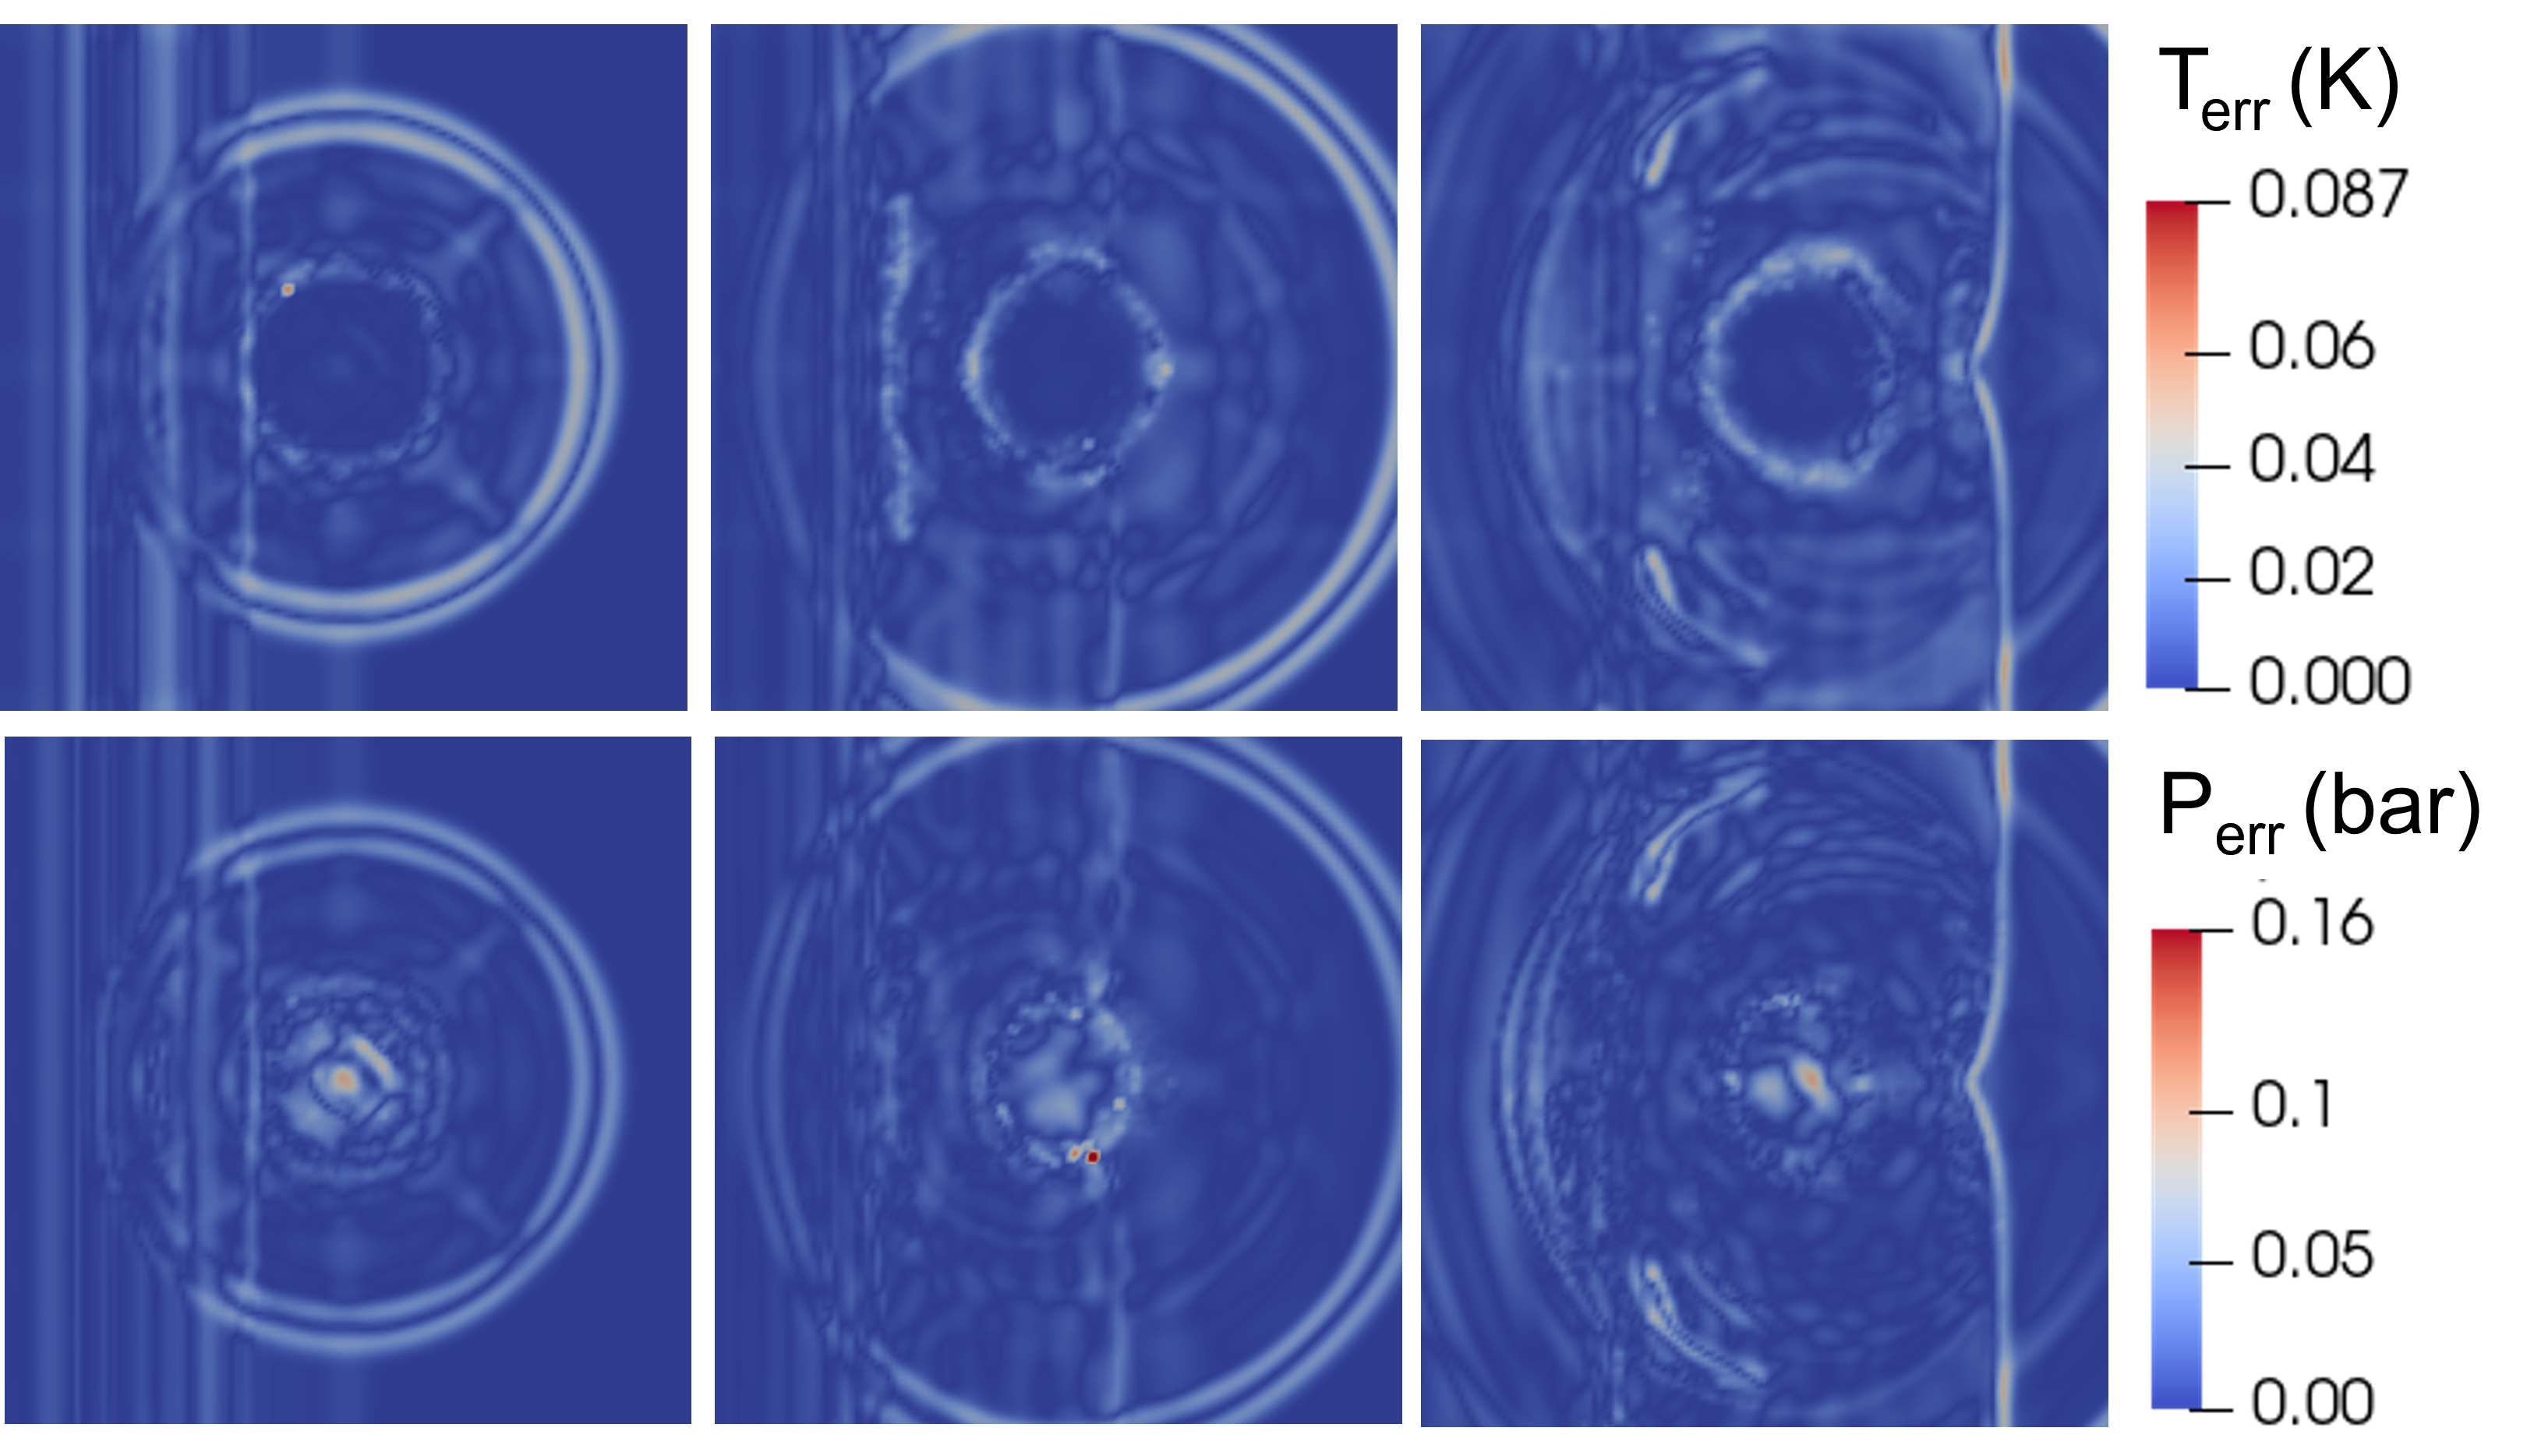
\includegraphics[width=0.8\linewidth]{3D_shock_1C_err_2.png}
	\caption{The error contours of the ISAT-VLE method in the 3D transcritical shock-droplet interaction simulation. From left to right are the time instants of $0.5\mu s$, $0.83\mu s$ s, and $1.2\mu s$. }
	\label{SD_3D_err}
\end{figure}

When the initial temperature is increased from 565 K to 620 K, the phase separation at the droplet interface changes significantly. Initially, as shown in Fig.~\ref{droplet_3d_1C_HT}, the two-phase indicator $\alpha$ indicates that the droplet interface is situated within the subcritical two-phase region. However, as the shock wave passes through the droplet, the interface transitions into the single-phase region, eventually leading to the complete disappearance of phase separation. This process is further illustrated in the P-T phase diagram depicted in Fig.~\ref{droplet_3D_1C_HT_phasediagram}. The data points of the initial condition lie within the phase boundary of the mixture of $X_{N_2}=0.7, X_{C_{12}H_{26}}=0.3$, confirming that the droplet interface is in the subcritical two-phase region. As the shock wave elevates the droplet's pressure, the thermodynamic conditions move outside of the phase boundary, resulting in the elimination of phase separation.

\begin{figure}[htbp]
	\centering
	\includegraphics[width=0.8\linewidth]{3D_shock_1C_HT_3_c.png}
	\caption{3D transcritical shock-droplet interaction simulation with an initial temperature of 620 K: the top figures are density, the bottom figures are $\alpha$, where $\alpha = \beta (1-\beta)$ is a two-phase interface indicator. From left to right are the time instants of $0.5\mu s$, $0.83\mu s$ , and $1.2\mu s$.}
	\label{droplet_3d_1C_HT}
\end{figure}


\begin{figure}[htbp]
	\centering
	\includegraphics[width=0.60\linewidth]{PT_1C_HT_2_p_c2.png}
	\caption{Phase diagram of the 3D transcritical shock-droplet interaction simulation with an initial temperature 600 K. Data points are taken from the time instance of $1.2\mu s$, when the shock wave has passed the droplet completely. The data points of the expansion wave are removed. The labels in the figure are mole fractions of \ce{N2}.}
	\label{droplet_3D_1C_HT_phasediagram}
\end{figure}

Next, we explore the behavior of a two-component droplet. In this simulation, the droplet consists of 60\% \ce{n-C12H26} and 40\% \ce{n-C8H18} (by mole). The initial temperature is set to 565 K, which is consistent with the first case in this section. In Fig.~\ref{droplet_3d_2C}, as the shock wave passes through the droplet, we observe the disappearance of part of the two-phase boundary. This is because \ce{n-C8H18} has a lower critical temperature of 568.9K compared to \ce{n-C12H26} (658.2 K), which changes the phase boundary (see Fig.~\ref{droplet_3D_2C_phasediagram}). In addition, a new phenomenon is observed: even after the shock wave completely passes through the droplet, some sections of the droplet interface remain in the two-phase region. This is attributed to the relatively low pressure in the wake region behind the droplet, allowing the interface to remain in the subcritical two-phase region. This reasoning is clearly depicted in the phase diagram of Fig.~\ref{droplet_3D_2C_phasediagram}, where the three-component system (\ce{n-C12H26}/\ce{n-C8H18}/\ce{N2}) exhibits a two-phase region overlapping with the low-pressure corner of the post-shock data points.

\begin{figure}[htbp]
	\centering
	\includegraphics[width=0.8\linewidth]{3D_shock_2C_2_c.png}
	\caption{3D transcritical shock-droplet interaction simulation with an initial temperature of 565 K, and the droplet consists of 60\% \ce{n-C12H26} and 40\% \ce{n-C8H18} (by mole): the top figures are density, and the bottom figures are $\alpha$, where $\alpha = \beta (1-\beta)$ is a two-phase interface indicator. From left to right are the time instants of $0.5\mu s$, $0.83\mu s$, $1.2\mu s$ .}
	\label{droplet_3d_2C}
\end{figure}

\begin{figure}[htbp]
	\centering
	\includegraphics[width=0.60\linewidth]{TP_2C_2_p_c2.png}
	\caption{Phase diagram of the 3D transcritical shock-droplet interaction simulation with an initial temperature of 565 K, and the droplet consists of 60\% \ce{n-C12H26} and 40\% \ce{n-C8H18} (by mole). Data points are taken from the time instance of $1.2\mu s$, when the shock wave has passed the droplet completely. The data points of the expansion wave are removed. The labels in the figure are mole fractions of \ce{N2}.}
	\label{droplet_3D_2C_phasediagram}
\end{figure}

The 3D transcritical shock-droplet interaction simulations with a single-component droplet and an initial temperature of 565 K were conducted using 128 CPU cores. The speed-up performance of the ISAT-VLE method is illustrated in Fig.~\ref{droplet_3D_perf}. Initially, the ISAT-VLE case exhibited a speed-up of approximately 33 times compared to the VLE case without ISAT. Even in the later stages, it still maintained a significant speed-up of 15 times. On average, the ISAT-VLE method achieved a speed-up factor of approximately 17, showing its effectiveness in accelerating the 3D VLE-based CFD simulations. Furthermore, it is evident that compared with the 3D transcritical TML simulation (as shown in Fig.~\ref{TML_3D_performace}), the computational workload difference between different regions is not as pronounced, making the results closer to those obtained from 2D simulations.


\begin{figure}[htbp]
	\centering
	\includegraphics[width=0.6\linewidth]{time_noISAT_new_2_m.png} 
	\caption{Speed-up performance of the ISAT-VLE method in the 3D transcritical shock-droplet interaction simulation.}
	\label{droplet_3D_perf}
\end{figure}

\section{parallel ISAT} \label{sec:pISAT}



%%A detailed combustion kinetic mechanism often includes tens to hundreds of species and hundreds to thousands of reactions. The simulation of complex flames (e.g., turbulent flames) requires solving many conservation equations, including detailed finite-rate chemistry, which demands a large amount of computational cost. To accelerate the computation, \textit{in situ} adaptive tabulation (ISAT) was introduced by Pope~\cite{pope1997computationally}.
%%ISAT is an on-the-fly tabulation method, in which records are dynamically added with additional information (e.g., the gradient of function). ISAT maintains error control by using finer granularity in regions of increased nonlinearity (shown in Fig.~\ref{ISAT_Schematic}). In a combustion simulation, the solution of chemical ordinary differential equations (ODE) is tabulated, which avoids a large amount of repeated computation and obtains a speed-up factor of about 1000 \cite{pope1997computationally}. ISAT has been successfully used in many combustion simulations \cite{pope1997computationally,gordon2007numerical,wang2003application,singer2006modeling,singer2004exploiting,tang2002implementation}. Moreover, several research works have been done to improve the algorithm. Chen improved performance by modifying search algorithm \cite{chen2004analysis}; Lu et al. implemented parallel ISAT in LES \cite{lu2005investigation}; Lu and Pope improved table searching strategies, error checking, and correction algorithms \cite{lu2009improved}; Blasi et al. extended ISAT to accelerate the simulation of complex heterogeneous chemical kinetics \cite{blasi2016situ}.

In the preceding section, we evaluated the performance of the ISAT-VLE model. We observed substantial acceleration in serial computation, yet encountered a decline in ISAT's performance when employing parallel computation. Given the imperative need to handle the extensive load of CFD calculations, parallel computing has become indispensable. Consequently, the diminished performance of ISAT in parallel computing scenarios imposes constraints on its applicability.Consequently, the diminished performance of ISAT in parallel computing scenarios imposes constraints on its applicability.

The original ISAT was not designed for parallel computation. When using original ISAT parallel computation, every process needs to maintain its own ISAT table and write repeated records into the table. Moreover, in simulations, substantial fluctuations in physical properties typically manifest in localized regions, such as shock waves and contact discontinuities. Compared to other regions, the computation in these regions tends to add more records in the ISAT table, often leading to pronounced imbalances when directly employing ISAT in parallel simulations. Researchers tried to address ISAT parallelization challenges in previous works\cite{lu2009computationally,wu2018parallel}, primarily by attempting to partition the computational workload within the computing domain into discrete chunks. They utilize the MPI communication mechanism to allocate these task chunks to individual MPI processes, ultimately achieving a more balanced distribution of computational load. However, their allocation method is fixed and unable to adapt to dynamically changing computing needs. The effectiveness of this approach hinges heavily on the spatial characteristics of the flow and the specific domain decomposition. Furthermore, the substantial volume of MPI communication involved can adversely impact ISAT performance.
Hence, it is difficult for existing methods to make full use of computing resources.


In this study, we proposed a parallel ISAT (see in Fig.~\ref{MPI_arch2}), which combines a shared-memory ISAT table with local ISAT tables and has a loading balancing algorithm to fully utilize the computation resources. Shared ISAT can fully utilize the computation results from individual processes, which enhances the perfoamce of load balancing algorithm. Shared-memory ISAT table is implemented using the shared memory in MPI-3. To work with the shared-memory architecture, a concurrent tree is developed to store the ISAT table and optimized for high-concurrency and high-performance reads, and low-concurrency writes.


\begin{figure}[htbp]
	\centering
	\includegraphics[width=0.9\linewidth]{MPI arch3.png}
	\caption{Schematic of the proposed parallel ISAT method.}
	\label{MPI_arch2}
\end{figure}

%a concurrency data structure (binary tree) to reduce the memory requirement and optimize the computing speed, and eventually improve the computational speed and accuracy in turbulent combustion simulation. The parallel ISAT is implemented using the shared memory in MPI-3. To work with the shared-memory architecture, a concurrent tree is developed to store the ISAT table and optimized for high-concurrency and high-performance reads, and low-concurrency writes. 2D counter-flow diffusion flame simulations are conducted to test the performance of parallel ISAT.

%%Lu et al. developed an ISAT extension for parallel computations by message passing among processes (i.e., MPI) \cite{lu2005investigation}. Therefore, it still cannot reduce redundant records, which wastes memory and limit the granularity of records.

%While ISAT has achieved excellent acceleration in computing, using detailed chemistry mechanisms is still challenging.  Parallel computing is critical to handle such a large amount of computation, but the original ISAT was not designed for parallel computation. In current approaches, every process needs to maintain its own ISAT table, solve the same chemical ODE, and write repeated records into the table. Lu et al. developed an ISAT extension for parallel computations by message passing among processes (i.e., MPI) \cite{lu2005investigation}. Therefore, it still cannot reduce redundant records, which wastes memory and limit the granularity of records.
%Besides parallel computing, the data structure in ISAT, binary tree, is not balanced and does not have a nearest neighbor search algorithm, which could affect performance. 
%%Hence, existing methods do not make full use of computing resources, which limits the ability of simulations to capture the small structures of turbulent flames or to use larger chemical mechanisms.


%In this study, we proposed a shared-memory parallel ISAT using a concurrency data structure (binary tree) to reduce the memory requirement and optimize the computing speed, and eventually improve the computational speed and accuracy in turbulent combustion simulation. The parallel ISAT is implemented using the shared memory in MPI-3. To work with the shared-memory architecture, a concurrent tree is developed to store the ISAT table and optimized for high-concurrency and high-performance reads, and low-concurrency writes. 2D counter-flow diffusion flame simulations are conducted to test the performance of parallel ISAT.
%An R-Tree is implemented in the concurrent tree rather than a binary tree used in the original method. Then, a faster search algorithm can be used for ISAT. The performance of parallel ISAT will be tested using a turbulent flame simulation.






\subsection{Method}
\subsubsection{shared memory architecture}
In the proposed model, the primary objective is to optimize the utilization of compute nodes' resources effectively. To achieve this goal, we need a hybrid distributed/shared model. While there are various approaches to implementing shared memory functionality, one common choice is the hybrid MPI-OpenMP model, which leverages OpenMP for shared memory support and MPI for process-level parallelism across nodes. The hybrid MPI-OpenMP model has gained significant traction and is widely employed in parallel computing environments \cite{ouro2019scalability,he2020structured,zhong2020efficient}.

In the MPI-3 standard, the MPI Shared Memory (SHM) \cite{brinskiy2017introduction} is introduced for supporting shared memory address space among MPI processes on the same node. With the MPI SHM model, an new hybrid programming approach combining MPI and the MPI Shared Memory (SHM) model emerges (hybrid MPI-MPI)\cite{hoefler2013mpi+}. Both MPI-MPI and MPI-OpenMP models can use the shared memory to reduce communication time in one node. However, many CFD solvers only use the pure MPI model rather than the MPI-OpenMP model. This is due to extra overheads from shared memory threading, hybrid MPI-OpenMP implementation may hardly outperform the pure MPI implementation \cite{rabenseifner2009hybrid}. For codes lacking OpenMP support, adopting the MPI-OpenMP model necessitates a comprehensive overhaul of the entire parallel structure to accommodate OpenMP. The use of the MPI-OpenMP model only requires incrementally adding OpenMP directives to the computationally intensive parts of the existing MPI code. However, given the complexity of modern large CFD code, such changes require a lot of careful debugging. In this regard, the hybrid MPI-MPI model proves more adaptable and portable.  It requires only minor adjustments to existing MPI code to introduce shared memory capabilities. Given this advantage, the MPI-MPI hybrid model are used in this work. Since the model is relatively new, there are still insufficient tutorials. we hope that this work can provide more experience in the use of the hybrid MPI-MPI model to help future developers.

When using the MPI model, we found the following three problems:
%The MPI SHM model is different from openMP in that MPI is inter-process communication. Each process has its own virtual memory space. This leads to three problems:



%1. 这使得同一个物理内存在不同进程下会出现不同的地址。这使得无法利用共享内存构建链表,树等复杂数据结构。
%2. 在MPI中,申请内存是一个collective call,申请共享内存需要所有核心一同完成,这使得在运行过程中动态分配内存会使性能退化到串行代码。
%3.而且由于同步的机制是为多线程设计的,这使得MPI共享内存的同步缺乏工具。
%我们提出了一个解决方案, 我们在一开始申请一整块内存,对于整块内存来说虽然在不同进程中地址不同,但是整块地址上的偏移量是相同的,我们使用相对于首地址的偏移量来代替地址。我们自己实现了slab allocator,来自己管理内存,共享内存只在代码开始运行时进行一大块内存。之后不在申请共享内存。

\begin{description}
	\item [1. Dynamic shared memory allocation] Dynamic shared memory allocation in the MPI model is a collective call executed by all processes, which means that a single process cannot allocate shared memory. However, when using the ISAT method, every processor should be able to update the table independently. If every update requires all the processes to allocate memory together, the efficiency of the whole system will be severely slowed down.
	\item [2. Memory address inconsistency] In modern operating systems, each process has its own virtual address space, which causes that for one block of physical memory, it can have different addresses in two processes. MPI SHM model is process-based rather than thread-based (in contrast, OpenMP is thread-based). Hence, the addresses of shared memory cannot be passed across processes, which makes the pointer cannot be used. ISAT is built based on a binary tree, which depends on the indexing method of the pointer.
	\item [3. Synchronization] Using shared memory, synchronization is important. If shared data are not protected properly, unexpected errors could happen, but most existing methods are designed for thread-based model.
	      %MPI standard does not provide flexible and efficient methods to protect shared memory.
\end{description}


When shared memory is employed solely for the purpose of optimizing the communication time of data blocks, the problems mentioned above do not come into play. However, when the objective extends to sharing intricate data structures and executing highly concurrent queries, it becomes imperative to address these shared memory-related issues. In response to these problems, we introduce a comprehensive set of memory management techniques:


\begin{description}
	\item [1.] Instead of allocating dynamic shared memory when needed, we allocate a big chunk of shared memory at the beginning, and we implemented a custom memory allocator (slab allocator \cite{bonwick1994slab}) to manage the shared memory. The slab allocator can provide efficient memory allocation for different sizes of objects and is now widely used by many Unix and Unix-like operating systems including FreeBSD and Linux.
	\item [2.] Although a memory Byte in two processes may have distinct virtual addresses, the address offsets between memory Bytes from the same block remain consistent across processes. This consistency enables us to employ the offset relative to the initial address of the entire memory block as new addresses that can be used by shared memory
	\item [3.] C++ provides build-in atomic variables. The synchronization for atomic variables is done at the instruction level. As a result, Atomic variables are safe in a multi-threading environment as well as a multi-process environment. Based on the atomic variable, mutual exclusion locks (mutex) are easy to implement. A mutex is a synchronization primitive: a mechanism that enforces limits on access to a resource when there are many threads/processes of execution. With mutexes, shared data can be protected from being simultaneously accessed by multiple threads/processes.

	      % which is free from data races; that is, if one thread writes to an atomic object while another thread reads from it, the behavior is well-defined. Although this technique is used on multi-thread rather than multi-process code, we tested and found atomic variables also work in MPI. Based on the atomic variable, mutual exclusion locks (mutex) are easy to implement. A mutex is a synchronization primitive: a mechanism that enforces limits on access to a resource when there are many threads of execution. With mutexes, shared data can be protected from being simultaneously accessed by multiple threads.
\end{description}

%



\subsubsection{Concurrent binary tree}
%%A challenge of developing the proposed shared-memory parallel ISAT is to ensure high efficiency and safety when manipulating the records in the table. A concurrent binary tree is implemented to ensure high performance. In simulations, most of the query can be directly retrieved from the table, which is a read operation. Write operations (growth and addition) are performed when the existing data is insufficient. %Since there are far fewer read operations than writes operations, the concurrent binary tree, needs to be optimized for high-concurrency and high-performance reads, and low-concurrency writes.
%%A challenge of developing the shared-memory ISAT is to ensure high efficiency and safety when manipulating the records in the table. A concurrent binary tree is implemented to ensure high performance. In simulations, most of the query can be directly retrieved from the table, which is a read operation. Write operations (growth and addition) are performed when the existing data is insufficient. Multiple reading operations can be performed simultaneously without causing corruption, but making writing operations paralleled is much more difficult. Improper ways can lead to unexpected errors. To ensure high efficiency and thread safety, the concurrent binary tree is designed to have the features below.

Developing a shared-memory ISAT presents a notable challenge: maintaining both high efficiency and data integrity when manipulating records within the table. To meet this challenge head-on, our solution incorporates a concurrent binary tree, a fundamental component that underpins the system's high-performance architecture.

In the simulations, the majority of queries involve read operations, where data is retrieved directly from the table. This read-heavy workload is well-suited for concurrent access, allowing multiple read operations to occur simultaneously without risk of data corruption. However, the complexity lies in parallelizing write operations (growth and addition). Implementing these write operations in a concurrent manner is considerably more intricate, as improper approaches can lead to unexpected errors and data inconsistencies.

To ensure both high efficiency and thread safety, the concurrent binary tree is meticulously designed with the following key features:

\begin{itemize}
	\item Reads are always lock-free (reading processes never block, even while writes are ongoing)
	      %\item Reading processes always see a consistent version of the tree
	\item Reading processes do not block writing processes
	\item Processes trying to write the same tree leaf block each other but never block reading threads
\end{itemize}

To realize the feature above, we employ a mutex mechanism to ensure the integrity of our shared-memory ISAT system during write operations. Notably, these write operations lock only the specific nodes affected at the lowest level of the tree. Consequently, multiple write operations can be simultaneously executed at distinct tree nodes, enhancing system efficiency and concurrency.  For better performance, the ISAT allows reads and writes to happen simultaneously. Three techniques are used:

%%To achieve the feature above, a mutex is used to block the node when a writing operation is executing. Since write operations only locks the affected node at the lowest level, multiple writing operation can be conducted at different tree nodes. As shown in the features, for better performance, the ISAT allows reads and writes to happen simultaneously. Three techniques are used for this purpose: 
\begin{description}
	\item [Atomic Restructuring Operation:] During writing, the structure of the binary tree needs to be accessible. Addition and growth operations are shown in Fig.\ref{MPI_op}. To preserve the structural integrity of the tree, updates that do not impact ongoing searches are prioritized (Fig.\ref{MPI_op}-2).  Subsequently, once all other updates are completed, the remaining modifications are executed through an atomic operation (Fig.\ref{MPI_op}-3). This process ensures that the tree structure remains consistently complete for concurrent read operations.

	\item [Copy-Based Data Modification:] Rather than directly update the data in place, all changes need to be first written to a new tree node or tree leaf, which is subsequently linked to the tree. Specifically, the ISAT's growth operation can be carried out by directly modifying a record. However, to safeguard data integrity, the updated result is first stored in a new leaf, which then replaces the original leaf (Fig.\ref{MPI_op}-1 Growth). This approach allows data modification to be transformed into a restructuring operation, and conducted atomically using the technique above.

	\item [Deferred Data Deletion:] Even after the removal of tree nodes and tree leaves, it is possible that some processes may still attempt to read this removed data. To accommodate such scenarios, deleted data is retained in its original form until all relevant read operations have been completed. Specifically,  the deleted red record (in Fig.\ref{MPI_op}-3 Growth operation) is preserved until it is no longer needed. All removed memory remains unchanged until the computation of the current time step has been finalized.
\end{description}




\begin{figure}[htbp]
	\centering
	\includegraphics[width=0.9\linewidth]{tree_update.png}
	\caption{Schematic of concurrent binary tree opration.}
	\label{MPI_op}
\end{figure}


Although the tree structure supports multiple writes and reads at the same time, memory allocator is still a bottleneck. To handle this, before each timestep, the allocator allocates a certain number of tree leaves and tree nodes for each process. In every timestep, we prioritize the utilization of pre-allocated memory, resorting to memory allocation through the allocator only when the pre-allocated memory is exhausted. This one-time allocation of a large memory block is exceptionally fast. By configuring an appropriate size for the pre-allocated memory, it becomes possible to eliminate the need for direct allocator usage in the majority of operations without incurring excessive memory waste. This approach helps maintain a high level of parallelism throughout the entire algorithm.

%%Using the above methods, we create a concurrent binary tree to store the ISAT table in each compute node. In this way, the data within a node can be centrally stored. Space wastage in multiple ISAT tables is avoided and unnecessary double calculations are reduced.

By employing the aforementioned approach, we establish a concurrent binary tree structure to store the ISAT table within each compute node. Through this method, all records within a node can be stored centrally, effectively mitigating space wastage in oringal ISAT method in which every process has its own ISAT table, and this way also reduces redundant calculations.

%使用上述方法,我们在每个计算节点建立一个Concurrent binary tree,用以存储ISAT table. 这样一来,一个节点内的数据都可以集中化的存储。避免了在多个ISAT表时的空间浪费,减少了不必要的重复计算。 

Regarding the redundant record deletion techniques discussed in the preceding section, implementing a highly concurrent linked list can prove challenging. Therefore, we opt for a simplified solution where we log the call timestamp after each record usage. Since identical timestamps are used for calls occurring within the same timestep, this approach effectively eliminates data race concerns without compromising performance. Periodically, at specified intervals of timesteps, we proceed to sort all records based on the timestamp and subsequently apply deletion criteria as previously defined.

In comparison to the original method, this approach has its drawbacks, particularly in terms of not being able to strictly guarantee conditions in every timestep. Additionally, the sorting operation encompasses all data, whereas the original method only affects incremental data. Consequently, this approach exhibits limitations when dealing with extensive data volumes. Nevertheless, given the well-controlled table size within this application, it does not impose a significant performance penalty.

%对于上一节提到的redundant record deletion methods,那个数据结构难以实现高并发的版本,因此我们使用了一个简化的版本,我们在每次使用一个记录后记录调用的时间,由于这种读写在同一个时间不长内被写入的值都是一样的,不存在数据竞争的问题,此过程不会降低速度。我们在每一定的时间步长后,根据最近调用的时间将所有的记录排序,然后使用之前相同的条件做删除。此方法相比于动态方法的缺点是,无法严格保证条件的满足,而且排序是针对所有数据的,动态方法是只对增量数据有改动。当数据量很大的时候这一方法会展现缺点,但是因为表格大小在此应用中控制的较好,不会带来明显的性能损失。



\subsubsection{Load balancing}


To handle load imbalance, some works \cite{lu2009computationally,wu2018parallel} They redistribute workload through MPI communication. However, their allocation method is fixed and unable to adapt to dynamically changing computing needs. Furthermore, the substantial volume of MPI communication involved can adversely impact ISAT performance.
%在并行的ISAT中

In contrast, our approach in this study involves sharing ISAT tables in memory, obviating the need to account for flow spatial characteristics and domain decomposition during task allocation. When distributing tasks, we bundle multiple tasks into batches (batch size is 100 in this work) and distribute them across the MPI processes to maximize the utilization of all available computing resources. The load-balancing algorithm employed is outlined as follows:

%在模拟中物理性质剧烈波动通常会集中在小区域内,比如激波,接触间断面,这些区域往往会为ISAT表中添加更多的记录。这使得在ISAT在并行时往往导致明显不平衡。ISAT的并行问题在一些工作里也被讨论过\cite{lu2009computationally,wu2018parallel},他们主要尝试将计算域内的计算量进行不同的划分,利用MPI通信机制重新分配给各个MPi进程,最终使得计算量更为均衡。这一方法的使用高度依赖计算流动空间分布上的特征,以及计算域的分解方法,并且大量的通信降低了ISAT的性能。由于在本工作中,我们将ISAT表在内存中共享,这使得在进行的分配任务时不需要考虑流动的空间特性。我们在分配任务时将多个任务打包,分发到不同的核心中,最大化的利用全部的计算资源。负载均衡算法如下:


We employ multiple linked lists using shared memory to efficiently handle load balancing. Specifically, we employ three key lists: List T, denoting ``task'', is responsible for storing pending task inputs awaiting allocation. Additionally, each process maintains its own List F, signifying ``finish'' to store the output results. When nodes in List F are used up, they are sent to List E, denoting ``empty'', and these nodes are then accessed by List T.

%When a node in List F are used and recycle to List E, denoting ``empty'', and  serves as a repository for available empty nodes,

Upon initialization, both List F and List T are left empty. List E is filled with nodes, with the number of nodes being three times the number of MPI processes. $N_{plan}$ is set to zero. In each time step, load balancing is shown in Algorithm~\ref{al:LB}.%During this initialization phase, each process is marked as not idle.

%每个进程的计算域内的问题被分成一定大小的batch, 我们取batch size 为100, 
%在计算中需要使用多个共享内存存储的链表队列。empty队列用于存储空的节点,filled用于存储等待被分配计算的任务。每个进程有一个complete队列,用于存储计算完的结果。在初始化时,filled队列与complete队列被置为空。empty队列放置3倍的MPI进程数的node
%每个进程初始化为不空闲。

%\begin{description}
%%    \item [1.] Complete the calculation of the next batch
%   \item [2.] Check whether the number of idle processes is greater than zero. If so, write the inputs of a certain number of batches of local tasks into List T. The number of batches is 2 times idle processes.
%检查空闲进程数是否大于零。如果是,将接下来2倍空闲进程数个本地任务batch的输入写入共享内存,将其插入filled队列。
%  \item [3.] Check whether list F for this process is empty. If the list is not empty, the task results are written to the corresponding computation domain, and the used node is inserted into list E.
%检查本进程的complete队列是否为空。如果不为空,将完成了的job结果写入本计算域的对应位置,完成后将队列插入empty队列。
% \item [4.] If all the batches have been computed or allocated, go to step 5, otherwise go back to step 1.
%如果所有的sbatch都被计算或被分配出去了,进入第5步,否则回到步骤一
%\item [5.] If this process is marked as idle and list T is not empty, fetched a batch from list T, finish the computing tasks, and place the result in the list F of the corresponding process.
%如果本进程标记为空闲且filled队列不为空,取出一个batch,求解job,然后将结果放入对应进程的complete队列中。
%\item [6.] Check whether list F for this process is empty. If the list is not empty, the task results are written to the corresponding computation domain, and the used node is inserted into list E.
%检查本进程的complete队列是否为空。如果不为空,将完成了的job结果写入本计算域的对应位置,完成后将队列插入empty队列。
%\item [7.] If the process is not idle, it is marked as idle, and the number of idle processes increases by one.
%如果进程不空闲,将其标为空闲,空闲进程数增加一。
%\item [8.] If the number of idle processes is equal to the total number of MPI processes, the results of all tasks of this process are written back and the list T is empty, the calculation ends. Otherwise, go back to step 5.
%如果空闲进程数等于进程总数,本进程全部任务的结果写入存储位置,且filled队列为空,结束计算,否则回到第5步
%\end{description}

%\begin{algorithmic}
%Complete the calculation of the next batch
%Check whether the number of idle processes is greater than zero. If so, write the inputs of a certain number of batches of local tasks into List T. The number of batches is 2 times idle processes.
%\end{algorithmic}   


\RestyleAlgo{boxruled}
\LinesNumbered
\begin{algorithm}[H]
	\caption{Load balancing algorithm} \label{al:LB}
	%List F and List T are left empty \;
	%List E is filled with $N$ empty nodes, $N = 3 \times N_{process} $ \;
	idle $\gets$ false, $N_{idle} \gets 0$\; \tcc{current process isn't idle, total number of idle processes is zero}
	$N_{send} \gets 0$, $N_{receive} \gets 0$\; \tcc{number of batches sent out and received are zero}
	\While{number of allocated batches $<$ number of total batches}{
		Complete the calculation of the next batch\;
		\If{$N_{send} < N_{plan}$}{
			write the inputs of one batch of local tasks into List T, $N_{send}$++\;
		}
		\If{$N_{idle} > 0$}{
			write the inputs of $ N_{idle}$ batches of local tasks into List T, $N_{send}$++\;
		}
		\If{list F of rank R is not empty}{
			the results are written back to the corresponding computation domain,
			the used node is inserted into list E\;
		}
	}
	\While{ idle = true \textbf{and} $N_{idle }=  N_{process}$ \textbf{and} list T is empty }
	{
		\If{idle = true \textbf{and} list T is not empty}{
			idle $\gets$ false,	$N_{idle}$--, $N_{receive}$++\;
			fetched a batch from list T,
			finish the computing tasks, 
			place the result in the list F of the sender's process\;
		}
		\If{list F of rank R is not empty}{
			the task results are written back to the corresponding computation domain\;
			the used node is inserted into list E\;
		}
		\If{idle = false}
		{
			idle $\gets $ true , $N_{idle} \gets   N_{idle}$ + 1\;
		}
	}
	$N_{plan} \gets N_{send} - N_{receive}$\; \tcc{update the number of batches plan to be sent in the next timestep}
\end{algorithm}



\begin{figure}[htbp]
	\centering
	\includegraphics[width=0.9\linewidth]{LB_chart.png}
	\caption{Schematic of load balancing algorithm}
	\label{MPI_LB}
\end{figure}

In Algorithm \ref{al:LB}, Line 3 to 14 constitute a local computation and task allocation loop.
Specifically, Lines 8 to 11 address the scenario where idle processes are available; in such cases, the process sends out $N_{idle}$ batches. This loop is triggered solely when idle processes exist. To minimize waiting times even further, we employ another loop (Line 5-6) where processes actively send the task based on the result of the previous time step. Line 15 to 27 encompass a loop for solving shared tasks and writing back the output. In simulation, the slow processes stay longer in the first loop, and the faster processes quickly complete their tasks and enter the second loop to share the computation tasks of the former, (see in Fig. \ref{MPI_LB}).  %Because the ISAT tables are shared among all processes, every process updates the same ISAT table, irrespective of the computational domain.
It's crucial to emphasize that linked list operations must address data race issues, necessitating the use of mutexes to guarantee the safety of each operation. Fortunately, these operations involve minimal computational overhead, resulting in negligible performance impact.
Through the method outlined above, all tasks can be equitably distributed across all processes, thereby maximizing the efficient utilization of computing resources.
%1-4是一个本地计算和任务transfer循环,5-8是求解被共享的任务,与将输出存储的循环。由于ISAT表是共享的,所以任何一个进程都能ISAT表都是相同的,不受计算域影响。需要强调的是队列操作需要处理数据竞争的问题,每次操作都需要用mutex保证操做的安全。这样的操作由于需要的计算量非常小,mutex的使用几乎不会产生对性能的影响。通过以上的方法所有任务可以被均匀的分配给所有的进程,最大化的利用计算资源。

\subsubsection{Distributed data structures}
%%Although we use a high efficiency concurrent binary tree, we can do multiple read and write operations at the same time. But the algorithms implemented to solve the data race problem are more burdensome, making simple read operations slower. To further improve performance, we implemented a distributed data structure that creates a local table per process while preserving the shared table. For retrieval operations, a process searches in the local table first. If the retrieval fails,it searches in the shared table. If a record in the shared table can be used for retrieval, add them to the local table. If the shared table also fails to retrieve, the growth operation and addition operation are tried again. For records that are newly added to the shared table, they are also inserted the local table as well. This approach makes use of local tables to improve the performance of query operations, while shared tables are used to maximize the utilization of the computation results of individual processes. This method allows each process to have a different local table, which is more suitable for dealing with the tasks from its own process. With this feature in mind, we count how many tasks in each batch have done growth and addition during the time step. In the next timestep, the batch that can be retrieved quickly is computed locally and the more time-consuming batch (conducted more growth and addition in previous time step) is sent out first.


While utilizing a high-efficiency concurrent binary tree, we enable concurrent read and write operations. However, addressing data race issues through implemented algorithms introduces added complexity, which impacts the speed of straightforward read operations. To further enhance performance, we've introduced a distributed data structure that incorporates both local and shared tables.

For a quary, each process initially try to retrieve using its local table. If this local query fail, it then resorts to the shared table. If a record within the shared table proves suitable for retrieval, it is subsequently added to the local table. In cases where even the shared table retrieval fails, we attempt growth and addition operations once more. Newly added records to the shared table are also inserted into the corresponding local tables.

This approach optimizes performance by leveraging local tables for speedy retrieval operations, while the shared tables maximize the utilization of computational results from individual processes. This method allows each process to maintain a distinct high-efficient local table tailored to its specific tasks. Capitalizing on this feature, we monitor the number of tasks in each batch that underwent growth and addition operations during the time step. In the subsequent time step, we prioritize processing the batch that can be quickly retrieved locally, while the more time-intensive batch (with more growth and addition operation in the previous time step) is sent out first.

%尽管我们使用了一个high efficiency concurrent binary tree,能够实现多个读和写的操作同时进行。但是为了解决data race的问题而实现的算法带来了更多的负担,这使得简单的读操作变的更慢。为了进一步提高性能,我们实现了一个distributed data structures,既在保留shared table的同时在每个进程再创建一个本地的table。在retrieval操作时首先在本地的table中搜索,如果失败则在shared table中搜索,对于shared table中的record要加入local table。如果shared table也没有成功 retrieve,则再尝试Growth operation和addition operation。 对于新加入shared table的record也要插入local table。这一方法利用了local table的来提高查询操作的性能,同时使用shared table来最大化利用各个进程的计算结果。不过这一方法使得每个进程有不同的local table,他们更适合处理自己进程的问题。考虑到这一特性,我们在每次计算后统计每个batch中有多少task进行了Growth和addition。在下一个timestep中优先本地计算那些能快速retrieve的batch,而优先把更为耗时的batch发送出去。


\subsection{Numerical test}
We conducted simulations of transcritical shock-droplet interactions to assess the performance of the proposed parallel ISAT method. These simulations were executed on a high-performance computing cluster comprising five nodes, each equipped with dual AMD EPYC 7702 processors, boasting a total of 128 cores per node.
\subsubsection{2D shock-droplet interaction simulations}

%我们使用了在之前章节使用的shock-droplet interation simulation,选取FC这一算力,对这一新模型的性能进行测试,首先我们测试了将计算域分为在x方向上分为两部分,两个MPI进程分别叫做P1,P2,
%We used the shock-droplet interaction simulation using the FC scheme in the previous chapter to test the performance of the new models. First, we used two processes to conduct the simulation. We decomposed the domain into two parts in the x direction. The two MPI processes are called P1 and P2, as shown in Fig.~\ref{MPI_P2}.

%%In Sec.\ref{sec:SD} section, we harnessed the power of the FC scheme to simulate the interaction between shockwaves and droplets. This simulation is also used to evaluate the performance of novel parallel ISAT models.

In Sec.\ref{sec:SD}, we simulated the interaction between shockwaves and droplets using the FC scheme. The same simulation (initial temperature 565 K, single component \ce{n-C12H26} droplet) is also used to evaluate the performance of novel parallel ISAT models. To carry out this investigation, we first conduct a simulation using two MPI processes. In the x-direction, we decomposed the domain into two distinct regions, aptly named P1 and P2, as illustrated in Fig.~\ref{MPI_P2}. We applied four ISAT methods for the simulation: the original ISAT approach (where each process generates its independent ISAT table), the shared ISAT approach, the shared ISAT with load balancing (LB), and the hybrid shared and local ISAT approach with LB.

\begin{figure}[htbp]
	\centering
	\includegraphics[width=0.6\linewidth]{P2_2.png}
	\caption{Schematic of comuputation domain in  two-process simulation}
	\label{MPI_P2}
\end{figure}



In Fig.\ref{MPI_2core}, we present the CPU time and memory consumption (in terms of table size) used during the execution of these simulations utilizing the three ISAT methods. In Fig.\ref{MPI_2core}(a), load imbalance is evident for both the shared ISAT and the original ISAT. This disparity starts at the initial encounter of the shockwave with the droplet in P1, occurring at approximately t1 (around 0.5 $\mu s$). This event precipitates a surge in computational workload within P1. Meanwhile, P2 remains unaffected until approximately 0.7 $\mu s$ (as denoted by t2 in Fig.\ref{MPI_2core}(a)), at which point the shockwave enters P2's computational domain, leading to an increase in computational demand. At roughly 1.5 $\mu s$, the shockwave's impact on P1 diminishes, subsequently reducing CPU time. The shared ISAT approach with LB makes good use of computing resources, and both processes achieve precisely equal CPU times. The hybrid shared and local ISAT approach's performance  has a similar performance compared to shared ISAT, but a little slower because of more computation required for local \& shared table management.

In order to compare parallel performance, we realize the slower process dictates the overall computational pace, necessitating that other processes wait until the slowest one completes its calculations. In each step, the slowest process determines the duration of computation. Comparing the three methods, we can see that the shared ISAT method shows better performance compared to the original ISAT. This improvement can be attributed to its ability to allow P1 and P2 to utilize each other's computation results, thereby mitigating redundancy. Moreover, the shared ISAT approach with LB further improves performance and minimizes load imbalance. Quantitatively, shared ISAT outperforms the original ISAT by 9.5\%, while shared ISAT with LB boasts a remarkable 34\% improvement in computational efficiency. The hybrid shared and local ISAT approach also achieves a 24\% improvement.


%我们使用三种方法分别进行模拟,分别是使用原先的ISAT(每个进程建立字节的ISAT表),共享的ISAT,共享的ISAT+ Load balancing (LB)。
%下图展示了我们使用三中方式进行模拟时,CPU time 与表格大小(内存消耗)。在a图上我们很清楚的看到,Shared ISAT 与 原先的ISAT有明显的不平衡。这一点也非常好理解,激波首先P1的区域内与液滴碰撞,导致计算量的增加,这是P2的计算域仍然是不受影响的,直到大约0.7mus时,激波进入P2的区域计算量开始增长。到大约1.5mus左右,P1内受激波的影响减少,CPU time 降低。可以看出shared ISAT比原先的ISAT性能有所提升,这是由于其共享特性P1,P2可以使用另一个进程的计算结果,减少了一些冗余计算。shared ISAT with LB 由于其算法特性导致两个进程的CPU时间完全一样。由于在并行中,较慢的进程是瓶颈,其他进程必须要等待直到最慢的进程完成。每个步长里最慢的进程是决定计算使用的时间。因此可以明显看到shared ISAT + LB 很明显的提高了计算速度。对于这个算例,shared总计算速度比ISAT快9.5\%,LB 比ISAT快34\%.
Fig.\ref{MPI_2core}(b) illustrates memory consumption through table size for three methods. In the original ISAT, we also provided separate table size data for process P1 and P2. Notably, the memory growth patterns for P1 and P2 align with CPU time growth. Around $1.5 \mu s$, P1's table size remains unchanged, which is because the redundant record deletion method works and limits the continued growth of table size.

The memory consumption of the two methods using the pure shared ISAT is similar. Throughout the entire computation process, the shared ISAT without LB consumes approximately 86\% of the memory space required by the original method, while with LB method, utilizes approximately 77\% of the original method's memory footprint. The hybrid shared and local ISAT approach entails a larger memory footprint, primarily attributed to the incorporation of local tables. However,  due to the presence of shared tables, the local tables only need to store a limited amount of frequently accessed data, resulting in a modest increase in memory usage. Consequently, the overall memory consumption remains 87\% of the original ISAT method.


%图b用table size展现了不同方法的内存消耗,在原先的ISAT中我们还额外画出了P1,P2两个线程分别的table size。P1,和P2的内存增长的区间很好地对应了CPUtime增长的部分。P1在1.5mus左右,table size 没有变化,这是因为redundant record deletion methods起作用了,限制了table size的继续增长。两个共享ISAT的方法的内存消耗比较接近。在整个计算中share方法与LB方法分别使用了原方法86\%,77\%的内存空间。

%下一部分,我们将算例分为四个进程,进一步观察分割方式对性能的影响

\begin{figure}[htbp]
	\centering
	\includegraphics[width=0.45\linewidth]{time_2core_n.png}
	\includegraphics[width=0.45\linewidth]{mem_2core_n.png}
	\caption{(a) The performance of different ISAT methods, in terms of the CPU time spent in every time step. (b) Memory usage of different ISAT methods, in terms of table size at every time step.}\label{MPI_2core}
\end{figure}

In the next part, we use four processes to further observe the effect of domain decomposition on performance.

%用4个MPI线程时,有三种常用的分解方式, 4x1 (在x方向分成4份,y方向分成一份,下同),2x2,1x4。 我们使用之前使用的三种IAST方法计算分别采用3种domain decomposition的方法模拟,得到9个结果。由于在之前的分析我们看到oringal ISAT和shared ISAT的不同进程在模拟中的CPU time趋势接近,我们在下图只展示oringal ISAT的结果。可以看到在4-1下,有两个进程几乎完全空闲,这是位于左右两侧的计算域,其中不含有液滴,于是内部的热力学状态十分简单,能够快速的查表计算。中间两个进程的情形比较接近之前两个进程的情形。在2-2下,这种情形相当于把上一节讨论两个进程的每个进程在在y方向均分,由于算例上下对称,这y方向分割,负载很均衡。在1-4下,最接近上下两侧的计算域完全不包含液滴,tabulation效率很高,只在reflection wave 进入其计算域时计算量提高。这三种方式里2-2的分割负载最为均匀。在shared ISAT with LB 中,三种分割方式对性能的影响明显较小。由于LB算法是有一定的开销的,2-2 这种更为均衡的分割方式性能更好一点。

When employing four MPI processes, there are three common strategies for decomposition: $4\times1$ (dividing the domain into four sections along the x-axis and one along the y-axis, the same applies below), $2\times2$, and $1\times4$. We conducted simulations utilizing all combinations of four ISAT methods and three decomposition techniques, resulting in a total of twelve outcomes. Given that our previous analysis showed similar CPU time trends between the original ISAT and shared ISAT during simulation, we present only the results for the original ISAT in Fig.~\ref{MPI_4core}.

Observations reveal that when using a $4\times1$ decomposition (Fig.~\ref{MPI_4core}(a)), two processes remain largely inactive, positioned on the left and right sides (along x direction) of the computational domain. These regions don't contain liquid droplets and thus exhibit a straightforward thermodynamic state conducive to efficient tabulation. The results of the middle two processes closely resemble those of previous simulations (see Fig.~\ref{MPI_2core}(a)). In the case of $2\times2$ decomposition  (Fig.~\ref{MPI_4core}(b)), this situation is very similar to the result of two processes. Because the computation domain of each process contains droplets, the computational load remains highly balanced.

In the $1\times4$ decomposition (Fig.~\ref{MPI_4core}(c)), the processes of the upper and lower domains contain no droplets. Consequently, tabulation efficiency is notably high. Additional computation is only required when the reflection wave enters their computational domain. Among the three decomposition methods, $2\times2$ achieves the most equitable load distribution. When employing shared ISAT with LB  (Fig.~\ref{MPI_4core}(d)), the three decomposition methods exert less influence on performance. Given that the LB algorithm incurs a certain level of overhead, the more balanced $2\times2$ decomposition method delivers better performance.

\begin{figure}[htbp]
	\centering
	\includegraphics[width=0.45\linewidth]{time_4core_4-1.png}
	\includegraphics[width=0.45\linewidth]{time_4core_2-2.png}

	\includegraphics[width=0.45\linewidth]{time_4core_1-4.png}
	\includegraphics[width=0.45\linewidth]{time_4core_lb.png}
	\caption{The effect of domain decomposition on the ISAT performance. (a)-(c) are the CPU time of 4 MPI processes using oringal ISAT in different domain decomposition: (a) $4\times1$, (b) $2\times2$, (c) $1\times4$. (d) the CPU time using share ISAT + LB in different domain decomposition}\label{MPI_4core}
\end{figure}

%下图展现了所有9个算例的总时间消耗,可以看出来shared ISAT 与origal ISAT 都明显的收到domain decomposition的影响,而且shared ISAT 并不总能获得相对于origal ISAT更好的性能。这是由于在shared ISAT中为了维护数据结构的完整防止data racing,我们设计的并发算法会降低一定性能,而且shared table使得table的大小增加,减慢搜索的速度。但是在shared ISAT with LB 中,性能受domain decomposition大大降低了。获得了明显的性能提升。

Fig.~\ref{MPI_4core_all} illustrates the total time consumption across all twelve results. It is evident that both shared ISAT and original ISAT are noticeably influenced by domain decomposition, and shared ISAT does not consistently outperform the original ISAT. This discrepancy arises from the fact that in shared ISAT, our concurrency algorithm, designed to maintain data structure integrity and prevent data racing, introduces some performance overhead. Additionally, the shared table increases in size, which can slow down search speeds.

%However, in the case of two method with LB, both methods are significantly faster and less affected by decomposition methods. There is no significant difference between the two methods, because the data race is not as obvious when the number of processes is small, and this difference will show up in subsequent tests with more processes.

Nonetheless, when considering the two methods with LB, it becomes evident that both approaches exhibit significantly improved performance and are less susceptible to the influence of decomposition methods.  Notably, there exists no substantial distinction between these two methods at this juncture. This absence of significant differentiation can be attributed to the fact that the data race issue is less pronounced when the number of processes is limited. It is expected that distinctions between the two methods will become more pronounced in subsequent tests involving a larger number of processes.
%domain decomposition leads to a significant performance boost. This improvement is particularly noteworthy and underscores the advantages of this specific configuration.


\begin{figure}[htbp]
	\centering
	\includegraphics[width=0.6\linewidth]{time_4core_all_n.png}

	\caption{The effect of domain decomposition on the ISAT performance. The bar chart shows total CPU time cost of simualtions using all combination of ISAT methods and decomposition methods}\label{MPI_4core_all}
\end{figure}

\subsubsection{3D shock-droplet interaction simulations}


%接下来我们测试方法的scaliity, 我们选取之前使用过的3D算例,使用128x128x128的网格,计算在8,16,32,64,128核时的性能。对比在分割时尽量选取使个个维度的分割份数相同(2-2-2,4-2-2,4-4-2,4-4-4,8-4-4)。

%接下来我们进一步测试新方法在使用核心数较多时的情况。我们选取之前使用过的3D算例,考虑到会使用较少的核心数计算,我们在保持其他设置不变的情况下使用一个更粗糙的网格(128x128x128)。我们使用8,16,32,64,128核模拟相同的算例,选用No ISAT, Orginal ISAT, shared ISAT with LB, hybrid shared & local ISAT 4种方法进行模拟。在做domain decomposation 是选用各个方向分割尽量均匀的方法(2-2-2,4-2-2,4-4-2,4-4-4,8-4-4, x-y-z)。 首先我们选取在128核时的情形进行分析


We conducted more testing to evaluate the performance of our new approach on a larger scale, utilizing a larger number of computing cores. For this assessment, we revisited the 3D shock-droplet interaction simulation with initial temperature 565 K and single component \ce{n-C12H26} droplet which is previously employed in Sec.\ref{sec:SD_3D}. However, due to the utilization of a reduced number of cores in certain simulations, we opted for a coarser mesh configuration with dimensions of $128\times128\times128$.  We maintained the other simulation settings identical to our previous runs.

Specifically, we executed simulations using 8, 16, 32, 64, and 128 cores for the same setting. We examined four methods for conducting the simulations: No ISAT, the original ISAT approach, shared ISAT with Load Balancing (LB), and the hybrid approach combining shared and local ISAT techniques Our choice of domain decomposition aimed to distribute computational work as evenly as possible in all directions. The domain decomposition configurations, progressing from 8 cores to 128 cores, were as follows: $2\times2\times2$, $4\times2\times2$,$ 4\times4\times2$, $4\times4\times4$, and $8\times4\times4$ (following the same notation as previously explained).

For our initial analysis, we focused on the scenario involving 128 cores. Fig.~\ref{MPI_128core}(a) illustrates the performance of the three ISAT methods. Within these curves, multiple peaks emerge between the 0.5 and 0.7 $\mu s$. This phenomenon arises due to the introduction of numerous new thermodynamic states into the entire system as the shock wave propagates through the droplet. Evidently, both the shared and hybrid ISAT methods effectively curtail computational costs once the shock wave has permeated the droplet, achieving and maintaining a consistently low level of computational overhead. In stark contrast, the original ISAT approach exhibits substantial fluctuations in computational requirements, consistently surpassing those of its counterparts.

During the initial 0.5 $\mu s$, only the shared ISAT method registers high computational costs. In this phase, the distribution of thermodynamic properties remains relatively simple, allowing for the completion of most calculations through rapid retrieval operations. However, owing to the expense associated with shared memory algorithms, the performance of the shared ISAT method suffers. In contrast, the hybrid ISAT method employs local ISAT to surmount this issue, significantly expediting calculations.

In comparison to the original ISAT approach, Shared ISAT and Hybrid ISAT achieve speedup factors of 1.32 and 4.95, respectively.

% 在图1中我们可以清楚的看到,三种ISAT方法的性能。三条曲线在0.5-0.7mu s 之间有多个峰值,这是在激波进入液滴时为整个系统的热力学引入了新的状态导致的。可以看到两个使用了shared ISAT的方法在激波进入液滴之后通过共享机制,将其他核心的计算成本降低,并维持在一个较低的水平。而original ISAT approach的计算量有较大的波动,并且高于其他的方法。在最开始的0.5mus里只有Shared ISAT的方法计算量较高,在这一阶段,热力学性质较为简单,可以通过快速的retrieval operation 完成绝大多数计算。但是由于共享内存算法的较高的计算成本使得计算大大提高了,而hybrid ISAT方法通过,local ISAT 克服了这一问题大大加速了计算。相对于original ISAT approach,Shared ISAT 与hybird shared & local ISAT 分别获得了speedup factor of 1.32, 4.95. 

Fig.~\ref{MPI_128core}(b) presents a comprehensive overview of the memory requirements. Notably, the memory demands for shared ISAT are exceptionally minimal. In fact, within the hybrid method, the shared table size remains within a similar magnitude as the former, but accompanied by the inclusion of 128 local tables, which significantly increases the overall table size. Nevertheless, even with this augmentation, the memory consumption of the hybrid method remains lower than that of the original method. Shared ISAT utilizes just 1/16 of the total size f original method, while hybrid ISAT occupies only 60% of the available memory space.

This observation highlights that each of the two new methods carries its own set of advantages and disadvantages. Shared ISAT excels in terms of memory efficiency, whereas hybrid ISAT boasts superior computational speed. Both approaches clearly outperform the original ISAT method in both temporal and spatial dimensions, offering enhanced performance across the board.


% 在图1展示了内存的的需求,纯shared ISAT的内存需求是最小的。实际上再hyrid 方法里,shared table 也非常小,与前者在一个量级上,但是128个local table 使得总table size大大增加。尽管如此,hyrbid 方法的内存消耗仍然小于 Original 方法。shared ISAT只使用了1/16的大小,hybird shared & local ISAT只也使用了60\%内存空间。可以看出两个新方法各有优劣,Shared ISAT 需要更小的内存,hybird shared & local ISAT 有更高的计算速度,并且他们在时间和空间两个维度上都明显好于original ISAT

%图中hybrid 方法的osillation是由于在此方法下shared table中的数据被访问的频率较低低,大量记录会因为不被访问的时长到达上限而被删除 (80 time step 这已设置也在之前被提及),于是导致table size 以设定的周期进行波动。

The oscillation pattern observed in Fig.~\ref{MPI_128core}(b) is attributed to the low-frequency data access within the shared table in the hybrid method. In this approach, a substantial number of records are removed when the unaccessed time surpasses the predefined upper limit (as previously set at 80 timesteps, as mentioned in Sec.\ref{sec:delete}). Consequently, the table size experiences periodic fluctuations as a direct consequence of this cyclic data management process. 


\begin{figure}[htbp] 
	\centering
	\includegraphics[width=0.45\linewidth]{time_test_128.png}
	\includegraphics[width=0.45\linewidth]{mem_core_128.png}
	\caption{(a) The performance of different ISAT methods of 3D shock-droplet interaction simulated using 128 cores, in terms of the CPU time spent in every time step (b) Memory usage of different ISAT methods, in terms of table size at every time step }\label{MPI_128core} 
\end{figure}




%接下来我们比较在不同核心数下的speed up factor与scalibility。 图2中更能展示了加速的效果。Shared ISAT已经获得了明显的加速效果,但是在Hybrid ISAT放下对比下仍显不足,hybrid ISAT将加速效果进行了巨大的提升,对从8核到128和的运算速度都带来了巨大的提升。即使在128核时仍然获得了30倍的加速。可以看到local table加入的额效果是惊人的,极大了提高了并行下的性能。图A展示了scalibility,可以看到Original ISAT is bad scaling, 从8核增加到128核的过程中,只加速了大约两倍。在使用了Shared之后,相对于从8核到128核加速了3倍左右。当hybrid方法使用时scalibility获得了明显的提升,加速了6倍。尽管这一scalibility任然无法达到No ISAT的水平已经获得了足够大的进步。

Fig.~\ref{MPI_parallel}(a) illustrates the acceleration effects of the ISAT method. Notably, the original ISAT exhibits impressive initial acceleration, providing a 30-fold speedup when utilizing 8 cores. However, it becomes evident that this acceleration effect diminishes as the core count increases. Shared ISAT delivers comparable performance at 8 cores with a more gradual decline in the speedup factor as core count increases, ultimately achieving a greater speedup factor compared to the Original ISAT. Despite the evident acceleration achieved by Shared ISAT, it remains somewhat modest in comparison to the remarkable gains realized through the hybrid ISAT method. Hybrid ISAT showcases a substantial surge in speed when scaling from 8 to 128 cores, obtaining an exceptional 30 times acceleration even with 128 cores engaged. This striking result underscores the incredible impact of incorporating a local table, significantly enhancing parallel performance.

Fig.~\ref{MPI_parallel}(b), focusing on scalability, accentuates the disparity among ISAT methods. Original ISAT exhibits suboptimal scaling, offering only a twofold acceleration when transitioning from 8 to 128 cores. Conversely, shared ISAT demonstrates a noteworthy improvement, achieving nearly a threefold speedup across the same core range. However, the Hybrid ISAT method takes scalability to new heights, achieving an impressive sixfold acceleration in this transition.

These comprehensive tests conclusively highlight the substantial performance enhancements achieved by employing both shared and local tables within the hybrid ISAT approach. Both in terms of scalability and absolute acceleration, the hybrid method vastly improves the parallel performance when compared to the original ISAT.


\begin{figure}[htbp] 
	\centering
	\includegraphics[width=0.45\linewidth]{time_parallel2.png} 
	\includegraphics[width=0.45\linewidth]{time_parallel.png}
	\caption{The speedup factor of different ISAT methods of 3D shock-droplet interaction simulated using 128 cores. (a) speedup factor compared to the 8-processor results using the same method (b) speedup factor compared to the No IAST using the same number of processors. }\label{MPI_parallel} 
\end{figure}
%%%%%%%%%%%%%%%%%%%%%%%%%%%%%%%%%%%%%%%%%%%%%%%%%%%%%%%%%%%%%%%%%%%%%%%%%%%%%%%%
